\documentclass[12pt,lot, lof]{puthesis}
\newcommand{\proquestmode}{}

%%%% Author & title page info %%%%
\def\rhrvTitle{Getting started with RHRV}
\title{\rhrvTitle}
\submitted{\today}  
\copyrightyear{2013}  
\author{Constantino A. Garc\'{i}a$^*$, Abraham Otero and Xos\'{e} Vila} 
    %   General parameters, for ALL pages:
    \renewcommand{\topfraction}{0.85}	% max fraction of floats at top
    \renewcommand{\bottomfraction}{0.6}	% max fraction of floats at bottom
    %   Parameters for TEXT pages (not float pages):
    \setcounter{topnumber}{2}
    \setcounter{bottomnumber}{2}
    \setcounter{totalnumber}{4}     % 2 may work better
    \setcounter{dbltopnumber}{2}    % for 2-column pages
    \renewcommand{\dbltopfraction}{0.66}	% fit big float above 2-col. text
    \renewcommand{\textfraction}{0.15}	% allow minimal text w. figs
    %   Parameters for FLOAT pages (not text pages):
    \renewcommand{\floatpagefraction}{0.66}	% require fuller float pages
  	% N.B.: floatpagefraction MUST be less than topfraction !!
    \renewcommand{\dblfloatpagefraction}{0.66}	% require fuller float pages
% The documentclass already sets parameters to make a high penalty for widows and orphans. 

%%%% Use packages %%%%
\usepackage{hyperref}
\hypersetup{bookmarksnumbered}
\usepackage{float}
\usepackage{listings}
\usepackage{placeins}
\usepackage{inputenx}
\usepackage{color}
\usepackage{textcomp}	
\definecolor{listinggray}{gray}{0.9}
\definecolor{lbcolor}{rgb}{1,1,1}
\lstset{
     backgroundcolor=\color{lbcolor},
     tabsize=4,
     rulecolor=,
	   basicstyle=\scriptsize,
     numbers=left,
     upquote=true,
     aboveskip={1.5\baselineskip},
     columns=fixed,
     showstringspaces=false,
     extendedchars=true,
     breaklines=true,
     prebreak = \raisebox{0ex}[0ex][0ex]{\ensuremath{\hookleftarrow}},
     frame=single,
     showtabs=false,
     showspaces=false,
     showstringspaces=false,
     identifierstyle=\ttfamily,
     keywordstyle=\color[rgb]{0,0,1},
     commentstyle=\color[rgb]{0.133,0.545,0.133},
     stringstyle=\color[rgb]{0.627,0.126,0.941},
}
\usepackage[acronym,nonumberlist]{glossaries}
\usepackage[font=small,format=plain,labelfont=bf,up,textfont=it,up]{caption}
\usepackage{pdfpages}
\usepackage{amsfonts}
\usepackage{amsmath}
\usepackage{geometry}
\usepackage{fancyhdr}
\usepackage{longtable}
\pagestyle{fancy}
\usepackage{graphicx}
\usepackage{verbatim}
\usepackage{multirow}
\usepackage{longtable}
\usepackage{booktabs}
% options of the bookstab package
\setcounter{secnumdepth}{4}
\setcounter{tocdepth}{4}
%set parameters for longtable:
% default caption width is 4in for longtable, but wider for normal tables
\setlength{\LTcapwidth}{\textwidth}
\ifdefined\printmode
  % Printed copy
  % url package understands urls (with proper line-breaks) without hyperlinking them
  \usepackage{url}
\else
\ifdefined\proquestmode

% ProQuest requires a double spaced version (set previously). They will take an 
% electronic copy, so we want links in the pdf, but also copies may be printed 
% or made into microfilm in black and white, so we want outlined links instead 
% of colored links.

% copy the already-set title and author to use in the pdf properties
\makeatletter
\hypersetup{pdftitle=\@title,pdfauthor=\@author}
\makeatother

\else
% Online copy
% adds internal linked references, pdf bookmarks, etc
% turn all references and citations into hyperlinks:
% -- not for printed copies
% -- automatically includes url package
% options:
% colorlinks makes links by coloring the text instead of putting a rectangle around the text.
\usepackage{hyperref}
\hypersetup{colorlinks,bookmarksnumbered}

% copy the already-set title and author to use in the pdf properties
\makeatletter
\hypersetup{pdftitle=\@title,pdfauthor=\@author}
\makeatother

% make the page number rather than the text be the link for ToC entries
%\hypersetup{linktocpage}
\fi % proquest or online formatting
\fi % printed or online formatting

%%%% end of the usepackage zone %%%%


%%%% Define commands %%%%

% Define any custom commands that you want to use.
% For example, highlight notes for future edits to the thesis
%\newcommand{\todo}[1]{\textbf{\emph{TODO:}#1}}

% create an environment that will indent text
% see: http://latex.computersci.org/Reference/ListEnvironments
% 	\raggedright makes them left aligned instead of justified
\newenvironment{indenttext}{
    \begin{list}{}{ \itemsep 0in \itemindent 0in
    \labelsep 0in \labelwidth 0in
    \listparindent 0in
    \topsep 0in \partopsep 0in \parskip 0in \parsep 0in
    \leftmargin 1em \rightmargin 0in
    \raggedright
    }
    \item
  }
  {\end{list}}

% another environment that's an indented list, with no spaces between items 
% -- if we want multiple items/lines. Useful in tables. Use \item inside the
% environment.
% \raggedright makes them left aligned instead of justified
\newenvironment{indentlist}{
    \begin{list}{}{ \itemsep 0in \itemindent 0in
    \labelsep 0in \labelwidth 0in
    \listparindent 0in
    \topsep 0in \partopsep 0in \parskip 0in \parsep 0in
    \leftmargin 1em \rightmargin 0in
    \raggedright
    }

  }
  {\end{list}}

%%%%%%%%%%%%%%%%%%%%%%%%%%%%%%%%%%%%%%%%%%%%%%%%%%%%%%%%%%%%%%%%%%%%%%%%%%%%%%%

%%%% Front-matter

% For early drafts, you may want to disable some of the frontmatter.
% Simply change this to "\ifodd 1" to do so.
\ifodd 0
% front-matter disabled while writing chapters
\renewcommand{\maketitlepage}{}
\clearpage
\newpage{\pagestyle{empty}\cleardoublepage}
\else
%\abstract{ % at the moment, we don't use abstract}

%\acknowledgements{
%I would like to thank...
%\input{acknowledgements}
%}

%\dedication{blabla. }

\fi  % disable frontmatter


%%%%%%%%%%%%%%%%%%%%%%%%%%%%%%%%%%%%%%%%%%%%%%%%%%%%%%%%%%%%%%%%%%%%%%%%%%%%%%
% 
\rhead{} % we don't use head for the pages
\usepackage{Sweave}
\begin{document}
% Sweave Figures will be stored on the figures folder, with the prefix "tutorial"
\Sconcordance{concordance:tutorial.tex:tutorial.Rnw:%
1 183 1 1 0 10 1 1 4 5 1}
\Sconcordance{concordance:tutorial.tex:././Chapters/ch-intro/chapter-intro.Rnw:ofs 201:%
1 111 1}
\Sconcordance{concordance:tutorial.tex:tutorial.Rnw:ofs 313:%
205}
\Sconcordance{concordance:tutorial.tex:././Chapters/ch-HRV/chapter-HRV.Rnw:ofs 314:%
1 513 1}
\Sconcordance{concordance:tutorial.tex:tutorial.Rnw:ofs 828:%
207}
\Sconcordance{concordance:tutorial.tex:././Chapters/ch-installation/chapter-installation.Rnw:ofs 829:%
1 6 1 1 2 4 0 1 2 3 1 1 2 4 0 1 2 1 1 1 2 4 0 1 2 42 1}
\Sconcordance{concordance:tutorial.tex:tutorial.Rnw:ofs 900:%
209}
\Sconcordance{concordance:tutorial.tex:././Chapters/ch-15guide/15guide.Rnw:ofs 901:%
1 1 1}
\Sconcordance{concordance:tutorial.tex:././Chapters/ch-15guide/sections/intro.Rnw:ofs 903:%
1 34 1 1 3 2 0 1 3 5 0 1 2 9 1}
\Sconcordance{concordance:tutorial.tex:././Chapters/ch-15guide/15guide.Rnw:ofs 957:%
4}
\Sconcordance{concordance:tutorial.tex:././Chapters/ch-15guide/sections/preprocessing.Rnw:ofs 958:%
1 10 1 1 2 1 0 1 1 3 0 1 2 21 1 1 6 13 0 1 2 15 1 1 2 8 0 1 2 9 1 1 2 9 %
0 1 2 7 1 1 4 12 0 1 2 6 1 1 2 4 0 1 3 4 0 1 2 19 1}
\Sconcordance{concordance:tutorial.tex:././Chapters/ch-15guide/15guide.Rnw:ofs 1114:%
6}
\Sconcordance{concordance:tutorial.tex:././Chapters/ch-15guide/sections/analyzing/analyzing.Rnw:ofs 1115:%
1 1 1}
\Sconcordance{concordance:tutorial.tex:././Chapters/ch-15guide/sections/analyzing/rawData.Rnw:ofs 1117:%
1 10 1 1 2 4 0 1 2 11 1 1 2 7 0 1 2 3 1}
\Sconcordance{concordance:tutorial.tex:././Chapters/ch-15guide/sections/analyzing/analyzing.Rnw:ofs 1157:%
4}
\Sconcordance{concordance:tutorial.tex:././Chapters/ch-15guide/sections/analyzing/analyzingTime.Rnw:ofs 1158:%
1 21 1 1 3 22 0 1 2 8 1 1 2 1 0 7 1 19 0 1 3 8 0 1 2}
\Sconcordance{concordance:tutorial.tex:././Chapters/ch-15guide/sections/analyzing/analyzing.Rnw:ofs 1250:%
6}
\Sconcordance{concordance:tutorial.tex:././Chapters/ch-15guide/sections/analyzing/analyzingFrequency.Rnw:ofs 1251:%
1 8 1 1 2 8 0 1 2 52 1 1 2 1 0 7 1 1 7 15 0 1 2 4 1 1 3 5 0 1 2 44 1 1 %
2 1 0 7 1 1 6 13 0 1 2 7 1 1 12 3 0 1 1 1 5 12 0 1 3 8 0 1 2 9 0 1 2 14 %
1 1 3 5 0 1 4 5 0 1 2 39 1}
\Sconcordance{concordance:tutorial.tex:././Chapters/ch-15guide/sections/analyzing/analyzing.Rnw:ofs 1538:%
8 1 1}
\Sconcordance{concordance:tutorial.tex:././Chapters/ch-15guide/15guide.Rnw:ofs 1540:%
8}
\Sconcordance{concordance:tutorial.tex:tutorial.Rnw:ofs 1541:%
211}
\Sconcordance{concordance:tutorial.tex:././Chapters/ch-advanced/advanced.Rnw:ofs 1542:%
1}
\Sconcordance{concordance:tutorial.tex:././Chapters/ch-advanced/sections/completing/completing.Rnw:ofs 1543:%
1 57 1 1 5 1 4 14 0 1 2 42 1 1 8 1 0 1 1 3 0 1 2 11 1 1 8 4 0 1 2 24 1 %
1 3 4 0 1 2 65 1 1 14 6 0 1 2 7 1 1 4 6 0 1 2 4 1 1 4 6 0 1 2 18 1}
\Sconcordance{concordance:tutorial.tex:././Chapters/ch-advanced/sections/advanced/advanced.Rnw:ofs 1832:%
1 3 1}
\Sconcordance{concordance:tutorial.tex:././Chapters/ch-advanced/sections/advanced/reading.Rnw:ofs 1836:%
1 13 1 1 3 5 0 1 2 22 1 1 2 1 0 1 1 1 2 14 0 1 2 5 1 1 3 5 0 1 2 2 1 1 %
2 1 0 1 1 3 0 1 2 31 1 1 2 1 0 1 1 1 2 14 0}
\Sconcordance{concordance:tutorial.tex:././Chapters/ch-advanced/sections/advanced/advanced.Rnw:ofs 1968:%
6 1 1}
\Sconcordance{concordance:tutorial.tex:././Chapters/ch-advanced/sections/advanced/intervals.Rnw:ofs 1970:%
1 34 1 1 2 1 0 2 1 1 2 9 0 1 2 1 4 6 1 1 2 1 0 1 2 4 0 1 3 1 0 1 2 4 0 %
1 2 23 1 1 2 1 0 1 3 2 0 1 3 5 0 1 2 60 1 1 2 1 0 2 1 1 2 13 0 1 2 12 1 %
1 2 1 0 1 1 1 2 13 0 1 2 13 0 1 1 6 0 1 1 10 0 1 2 15 1 1 3 10 0 1 1 10 %
0 1 2 1 1 1 2 6 0 1 1 5 0 1 1 6 0 1 2 6 1 1 2 6 0 1 1 12 0 1 1 5 0 1 1 %
6 0 1 2 9 1 1 3 8 0 1 2 8 0 1 2 11 0 1 2 7 0 1 2 6 0 1 2 7 0}
\Sconcordance{concordance:tutorial.tex:././Chapters/ch-advanced/sections/advanced/advanced.Rnw:ofs 2380:%
9 1 1}
\Sconcordance{concordance:tutorial.tex:././Chapters/ch-advanced/sections/advanced/readSave.Rnw:ofs 2382:%
1 4 1 1 2 9 0 1 2 8 1 1 2 4 0 1 2 9 1 1 2 8 0 1 2 2 1}
\Sconcordance{concordance:tutorial.tex:tutorial.Rnw:ofs 2433:%
213 19 1}
 
\setlength{\parindent}{0pt}
\makefrontmatter

% Create table of glossaries and acronyms
\makeglossaries
\printglossary[type=\acronymtype] 

% Load RHRV for all the examples

%%%%%%%%%%%%%%%%%%%% Table of glossaries and acronyms %%%%%%%%%%%%%%%%%%%%%%%%%%
\newacronym{ANS}{ANS}{Autonomic Nervous System}
\newacronym{STFT}{STFT}{Short Time Fourier Transform}
\newacronym{niHR}{niHR}{Non Interpolated Heart Rate}
\newacronym{HRV}{HRV}{Heart Rate Variability}
\newacronym{HR}{HR}{Heart Rate}
\newacronym{SA}{SA}{sinoatrial node}
\newacronym{VLF}{VLF}{Very Low Frequency}
\newacronym{LF}{LF}{Low Frequency}
\newacronym{HF}{HF}{High Frequency}
\newacronym{RSA}{RSA}{Respiratory Sinus Arrhythmia}
\newacronym{ULF}{ULF}{Ultra Low Frequency}
\newacronym{ECG}{ECG}{electrocardiogram}
\newacronym{FFT}{FFT}{Fast Fourier Transform}
\newacronym{DFT}{DFT}{Discrete Fourier Transform}
\newacronym{DWT}{DWT}{Discrete Wavelet Transform}
\newacronym{MODWT}{MODWT}{Maximal Overlap Discrete Wavelet Transform}
\newacronym{DWPT}{DWPT}{Discrete Wavelet Packet Transform}
\newacronym{MODWPT}{MODWPT}{Maximal Overlap Discrete Wavelet Packet Transform}
\newacronym{bpm}{bpm}{beats per minute}
\newacronym{SDNN}{SDNN}{Standard Deviation of the NN interval}
\newacronym{SDANN}{SDANN}{Standard Deviation of  the Average NN/(RR) intervals calculated over short
 periods}
\newacronym{RMSSD}{RMSSD}{root mean square of successive differences}
\newacronym{SDNNIDX}{SDNN index}{the mean
of the standard deviation calculated over the windowed RR intervals}
\newacronym{pNN50}{pNN50}{proportion of successive RR intervals greater than 50 ms}
\newacronym{MADRR}{MADRR}{median of the absolute values of the successive differences between the RR intervals}
\newacronym{TINN}{TINN}{triangular interpolation of NN (RR) interval histogram}
\newacronym{PSD}{PSD}{power spectrum density}
%%%%%%%%%%%%%%%%%%%%%%%%%%% Chapters %%%%%%%%%%%%%%%%%%%%%%%%%%%%%%%%%%%%%%%%%%
% Use SweaveInput for clearness
%%%%% New chapter %%%%%%
% !Rnw root = ../../tutorial.Rnw
\chapter{Overview\label{ch:overview}}
It has been recognized in the past two decades that there is a significant 
relationship between the \gls{ANS} and cardiovascular mortality, including 
sudden cardiac death. Experimental evidence for a connection between a 
propensity for cardiac failure and either increased sympathetic or reduced
parasympathetic activity has encouraged the search of quantitative markers of
autonomic activity.\\

One of the most promising non-invasive markers is \gls{HRV}. \gls{HRV} refers
to the variation over time of both the intervals between consecutive heart beats
and the instantaneous \gls{HR}. As the heart rhythm is modulated by the
\gls{ANS}, \gls{HRV} is thought to reflect the activity of the sympathetic and 
parasympathetic branches of the \gls{ANS}. The continuous modulation of the
ANS results in continuous variations in heart rate. \gls{HRV} has been 
recognized
to be a useful non-invasive tool as a predictor of several pathologies such as
myocardial infarction, diabetic neuropathy, sudden cardiac death and ischemia,
among others \cite{kautznerClinical}. \\

The existence of several software tools (Kubios HRV \cite%
{kubios}, the \gls{HRV} toolkit for MatLab \cite{matlab} or aHRV
\cite{ahrv}, just to mention a few) have helped to popularize its use. Some of 
these software packages are commercial and require the purchase of expensive 
licenses (e.g., aHRV). Others while they are free, they require the purchase of 
expensive commercial software on which they depend (e.g., the HRV toolkit for 
MatLab).  Kubios is free (though not open source), but it is based on a 
graphical user interface, which makes it extremely tedious to perform 
systematic analyses of a large database of recordings, as the user must 
manually load and analyze through the user interface each recording.  In this 
context, we have developed RHRV, an open-source package for the statistical 
environment R \cite{waveletBiosignals}, \cite{waveletArticle}, \cite{vilaRHRV}, 
\cite{vila2009r}. To the best of our knowledge, RHRV is the only completely 
free and open source software package for performing HRV analysis and that is 
based on scripting commands; thus it enables the easy automation of analyses of 
a large number of 
recordings. \\

RHRV provides a complete set of
tools for \gls{HRV} analysis which can be used for developing new \gls{HRV} 
analysis algorithms or for performing clinical experiments. Although this 
software is 
mainly designed for the analysis of the \gls{HRV} in humans, it may also be 
used by animal researchers. Among the main characteristics of RHRV, we may 
highlight:
\begin{itemize}
\item RHRV can read heart rate data in multiple formats such as ASCII, Polar, 
Suunto and WFDB.
\item RHRV can compute the \gls{HRV} time series from the beats positions as 
well as preprocessing  and filtering the \gls{HRV} time series to eliminate 
outliers or spurious points.
\item RHRV includes functionality for the visualization and manipulation of the 
\gls{HRV} time series.
\item RHRV includes the most commonly \gls{HRV} analysis techniques, with 
facilities for tuning the most important analysis parameters. It is possible to:
	 \begin{itemize}
	 	\item Perform time-domain analysis.
		\item Perform frequency-domain analysis; they provide 
information on the renin	-angiotensin system (Very Low Frequency 
component), both sympathetic and
		parasympathetic systems (Low Frequency component) and the 
parasympathetic system (High Frequency component). The components can be 
calculated using both Fourier analysis
		and wavelet analysis.
		\item Perform nonlinear analysis techniques; they can extract 
some valuable information from the \gls{HRV} since it responds to a complex 
control
		system.
	 \end{itemize}
\item RHRV can	 split \gls{HRV} series into different segments that may 
correspond with different pathological states (i.e.: \gls{HRV} inside and 
outside apnea episodes). This simplifies
the statistical comparison of the heart rate inside and outside episode events.
\item RHRV provides flexibility for accessing directly the internal data 
structures that it uses in its calculations.
\end{itemize}

The RHRV package can be freely downloaded from the R-CRAN repository 
\cite{cran}. \\
\section{Aim} The aim of this tutorial is to help the user to get started with 
the RHRV package for the R environment. This document supposes that the user 
has some basic knowledge about the R environment as well about \gls{HRV}. 
However, a short introduction to \gls{HRV} will be given, and further 
references are provided.

\section{Structure of the document} The remainder of this document is 
structured as follows. First, a brief review of several \gls{HRV} topics is 
given in Chapter \ref{ch:HRV}. This chapter contains a short discussion on the 
physiological origins of heart rate variability, as well as a review of the 
frequency
components of \gls{HRV}. Section \ref{sec:obtainingHRV} continues discussing 
the extraction of heart beat periods. The derivation and the preprocessing of 
\gls{HRV} time series are also described.  In Section \ref{sec:analysisTechn}, 
the most common \gls{HRV} analysis methods are summarized (although they will 
be be covered in more depth when they are introduced in the document). The 
descriptions
of the methods are divided into time-domain, frequency-domain, and nonlinear. A 
discussion on the important issue of stationarity is included. The rest of the 
chapter (Section \ref{sec:pathologies}) is focused on the use of \gls{HRV} as a 
predictor of different pathologies and its clinical applications.\\

Chapter \ref{ch:installation} explains how get RHRV installed in your computer. 
This guide assumes that you have already installed R on your computer.\\

Chapter \ref{ch:Quick} presents a ``15-minutes guide to RHRV''. This chapter 
presents the essential functions needed to perform some basic analysis with 
RHRV. Chapter \ref{ch:RHRV} completes the functionality introduced in chapter 
\ref{ch:Quick} and presents more advanced features available in RHRV. Although 
there exist some functionality in the RHRV package for performing nonlinear 
analysis of a \gls{HR} signal, this current version of the tutorial will not 
treat these functions. Future versions of this tutorial will deal with this 
functionality.
%%%%% New chapter %%%%%%
% !Rnw root = ../../tutorial.Rnw
\chapter{Heart Rate Variability\label{ch:HRV}}

Heart Rate Variability (\gls{HRV}) describes variations over time of both 
instantaneous \gls{HR} and  the intervals between consecutive heart beats.
The rhythm of the heart is modulated by the \gls{SA}, which is largely 
influenced by both
the sympathetic and parasympathetic branches of
the \gls{ANS} (see Figure \ref{fig:influencia}). Sympathetic activity increases 
the heart rate and its response is slow (a few seconds). On the other
hand the Parasympathetic activity decreases the heart rate and its response is 
faster (0.2-0.6 seconds). Parasympathetic influence
on heart rate is mediated by the action of the vagus nerve. 
There are also some feedback mechanisms modulating the heart rates, that try to 
maintain cardiovascular
homeostasis by responding to the perturbations sensed by baroreceptors and 
chemoreceptors.\\


Under resting conditions, vagal tone prevails. However, parasympathetic and 
sympathetic activity constantly interact. The continuous modulation of the 
\gls{ANS} results in continuous variations in heart rate as shown in Figure 
\ref{Fig:varhr}. The beat to beat interval variations are the result of the 
interaction of the beat-to-beat control mechanisms.\\

Due to the different speed of response of both branches of the \gls{ANS}, it is 
possible to use the frequency analysis to discriminate between the sympathetic 
and parasympathetic contributions to the \gls{HRV}. Akselrod et 
al.\cite{akselrod1981} described three components in the \gls{HRV} power 
spectrum
with physiological relevance: the \gls{VLF} component (frequencies below 0.03 
Hz),
the \gls{LF} component (0.03-0.15 Hz) and the \gls{HF} component
(0.15-0.4 Hz). However, at present there is no absolute consensus on the 
precise limits of their
boundaries.\\



\begin{figure}[H]
\begin{center}
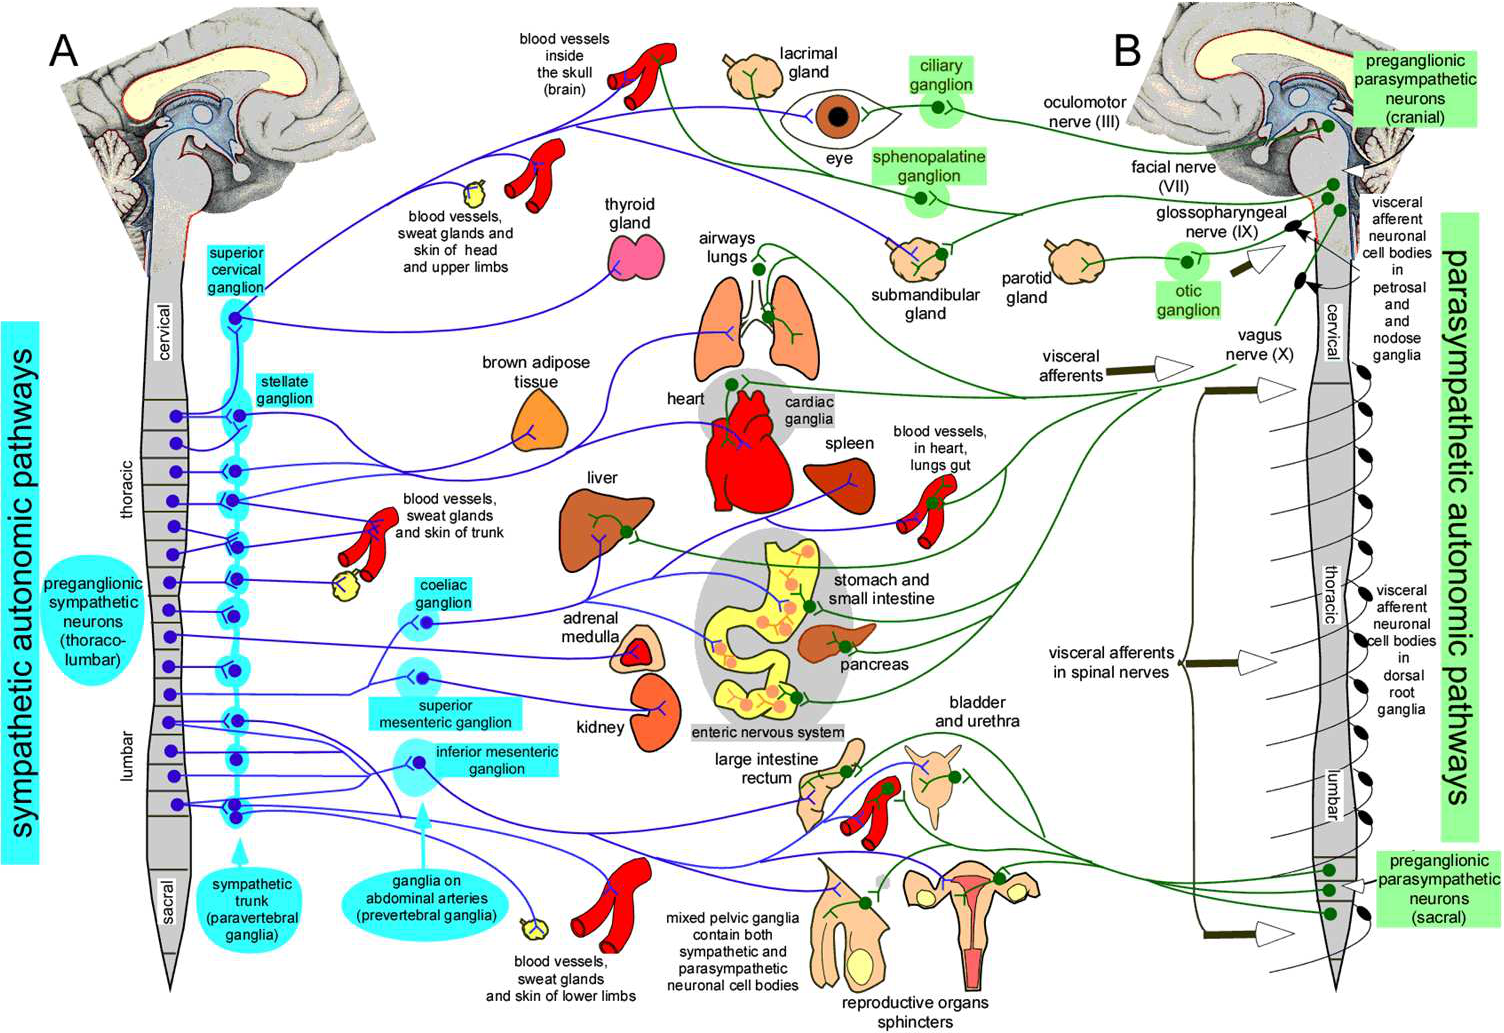
\includegraphics[angle=90,height=7in]{figures/influencia.pdf}
\caption[Modulation of the heart rate by the ANS]{\label{fig:influencia} 
Modulation of the heart by the sympathetic and parasympathetic systems. Figure 
taken from \cite{ansScholar}.}
\end{center}
\end{figure} 



\begin{figure}[h]
\begin{center}
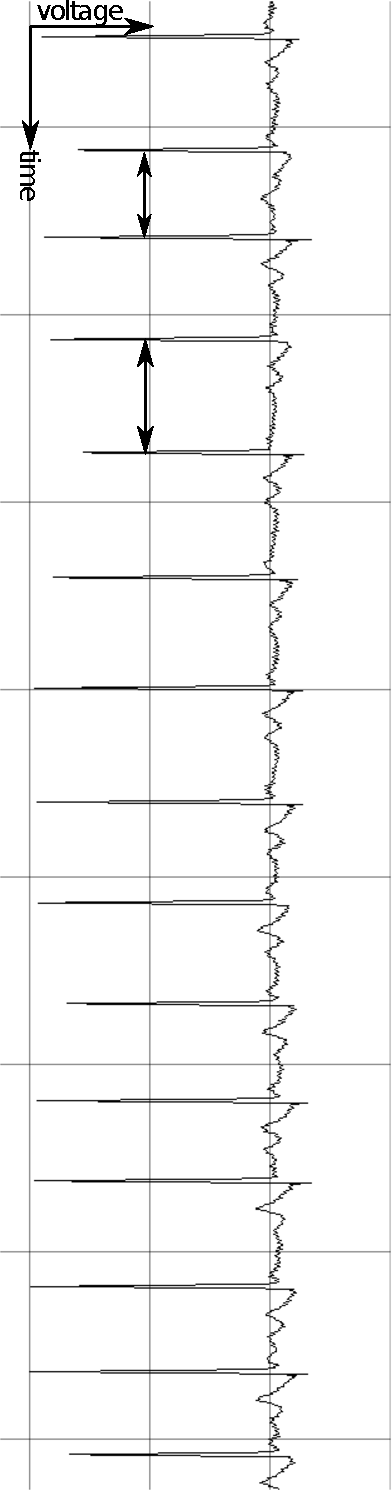
\includegraphics[width=0.2\textwidth,angle=90]{figures/varhr.pdf}
\caption[Heart rate variation]{\label{Fig:varhr} Heart rate variation as a 
consequence of the modulation of the ANS.}
\end{center}
\end{figure}

Among all the \gls{HF} mechanisms involved in the heart rate modulation we find 
the so called
\gls{RSA}: the heartbeat synchronization with the respiratory rhythm 
\cite{berntson1997}. In addition to the breathing frequencies, the \gls{HF}
component is believed to be of parasympathetic origin. It should be noted that, 
although it is common to set the upper limit of the \gls{HF} band to 0.4-0.5 
Hz, it may extend up to 1 Hz for children or adults during exercise.\\

The \gls{LF} component is a subject of controversy.  Some \cite{akselrod1981}, 
\cite{appel1989beat} consider that the \gls{LF} phenomena is  of both
 sympathetic and parasympathetic origin, although some authors have suggested 
that the sympathetic system predominates \cite{kamath}, \cite{malliani}.
This discrepancy is due to the fact that, in conditions of sympathetic 
excitation, a decrease in the absolute power of the \gls{LF} band is observed. 
This band also includes the component referred
 to as the 10-second rhythm or the Mayer wave, caused by oscillations in 
baroreceptor and chemoreceptor reflex control systems.\\
 
Spectral analysis of 24-hour recordings  \cite{24hrecords}, \cite{malliani} 
shows that in healthy individuals 
both \gls{LF} and \gls{HF} bands exhibit a circadian pattern and reciprocal 
fluctuations, with higher values of the \gls{LF} in the
daytime and of \gls{HF} at night.\\

\gls{LF} and \gls{HF} power can increase under different conditions. An 
increase of \gls{LF} is observed during mental stress, standing and
moderate exercise in healthy subjects, and during hypotension, physical 
activity and occlusion of a coronary artery or common
carotid arteries in conscious dogs. On the other hand, an increase of the 
\gls{HF} activity is observed during cold stimulation of the
face, rotational stimuli and controlled respiration \cite{forceHRV}.\\

 
The LF/HF ratio is often used by some investigators \cite{forceHRV} as a 
quantitative mirror of the sympatho/vagal balance. However,
other researchers disagree about the usefulness of the LF/HF index 
\cite{berntson1997}.\\

Finally, the rhythms associated with \gls{VLF} have not been studied as deeply 
as the higher frequencies. Indeed, some authors doubt that there there is a 
specific physiological process attributable to these heart period changes. 
Furthermore, the VLF band is affected by algorithms  of baseline removal 
\cite{forceHRV}. Despite all these objections, some authors have related the 
\glslink{VLF}{Very Low Frequency} with the renin-angiotensin system. Finally, 
it is possible to split this band into another two: the Very Low Frequency Band 
(\gls{VLF}, 0.003-0.03 Hz) and the \gls{ULF} Band(0-0.003 Hz).
Unless explicitly mentioned, the \gls{VLF} band will be used to refer the  (0 - 
0.03 Hz) band.\\

Figure \ref{fig:hrvSpectrum} summarizes the influence of the \gls{ANS} system 
over the different \gls{HRV} frequency bands.\\

%%%%%%%%%%%%%%%%%%%%%%%%%%%%%%%%%%%%%%%%%%%%%%%%%%%%%%%%%%%%%%%%%%%%%%%%%%%%%%%%
%%%%%%%%%%%%%%%%%%%%%%%%%%%
\begin{figure}[ht]
\begin{center}
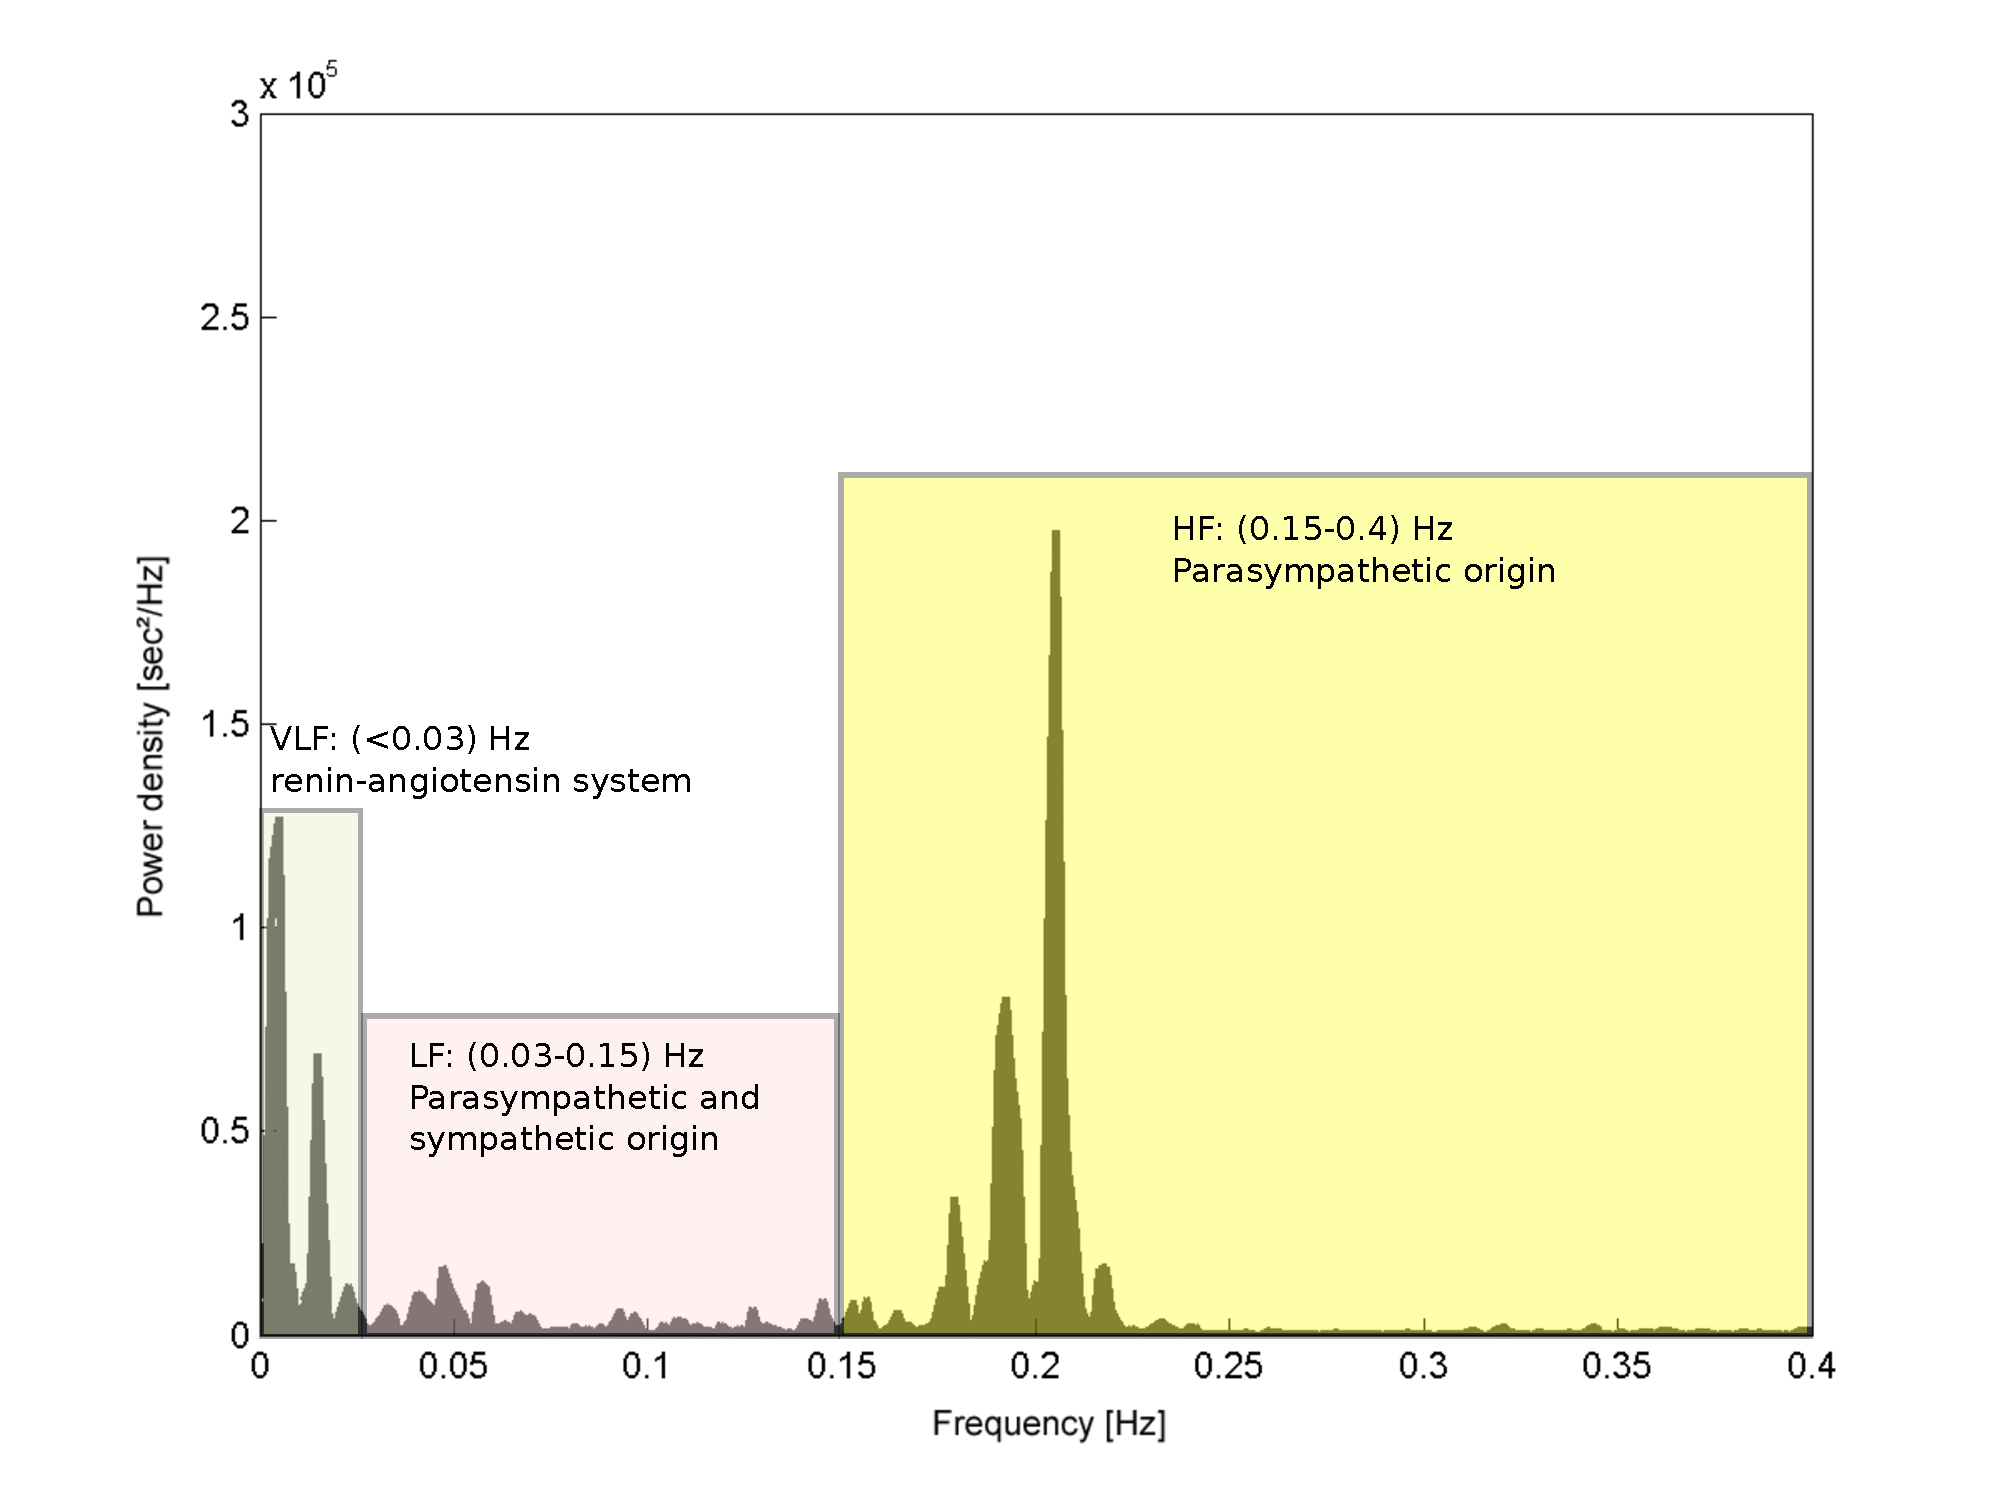
\includegraphics[scale=0.4]{figures/hrvSpectrum.pdf}
\caption{\label{fig:hrvSpectrum} Influence of the ANS system over the different 
HRV frequency bands.}
\end{center}
\end{figure} 
%%%%%%%%%%%%%%%%%%%%%%%%%%%%%%%%%%%%%%%%%%%%%%%%%%%%%%%%%%%%%%%%%%%%%%%%%%%%%%%%
%%%%%%%%%%%%%%%%%%%%%%%%%%%

\section{Obtaining HRV time series\label{sec:obtainingHRV}}
\subsection{QRS detection\label{QRS-detection}}

The aim of \gls{HRV} analysis is to analyze the sinus rhythms while it is 
modulated by the \gls{ANS}.  Thus, the starting point for \gls{HRV} analysis 
should be the extraction of the SA-node action potentials from the \gls{ECG}.
A typical \gls{ECG} showing a heartbeat consists of a P wave, a QRS complex and 
a T wave (see Figure \ref{fig:ecg}). The P wave represents the wave of 
depolarization that spreads from the SA-node throughout the atria. 
The QRS complex reflects the rapid depolarization of the right and left 
ventricles. Since the ventricles are the largest part of the heart, in terms of 
mass, the QRS complex usually has a much larger amplitude than the P-wave. The 
T wave represents the ventricular repolarization of the ventricles.
On rare occasions, a U wave can be seen following the T wave. The U wave is 
believed to be related to the last remnants of ventricular repolarization.\\

%%%%%%%%%%%%%%%%%%%%%%%%%%%%%%%%%%%%%%%%%%%%%%%%%%%%%%%%%%%%%%%%%%%%%%%%%%%%%%%%
%%%%%%%%%%%%%%%%%%%%%%%%%%%
\begin{figure}[ht]
\begin{center}
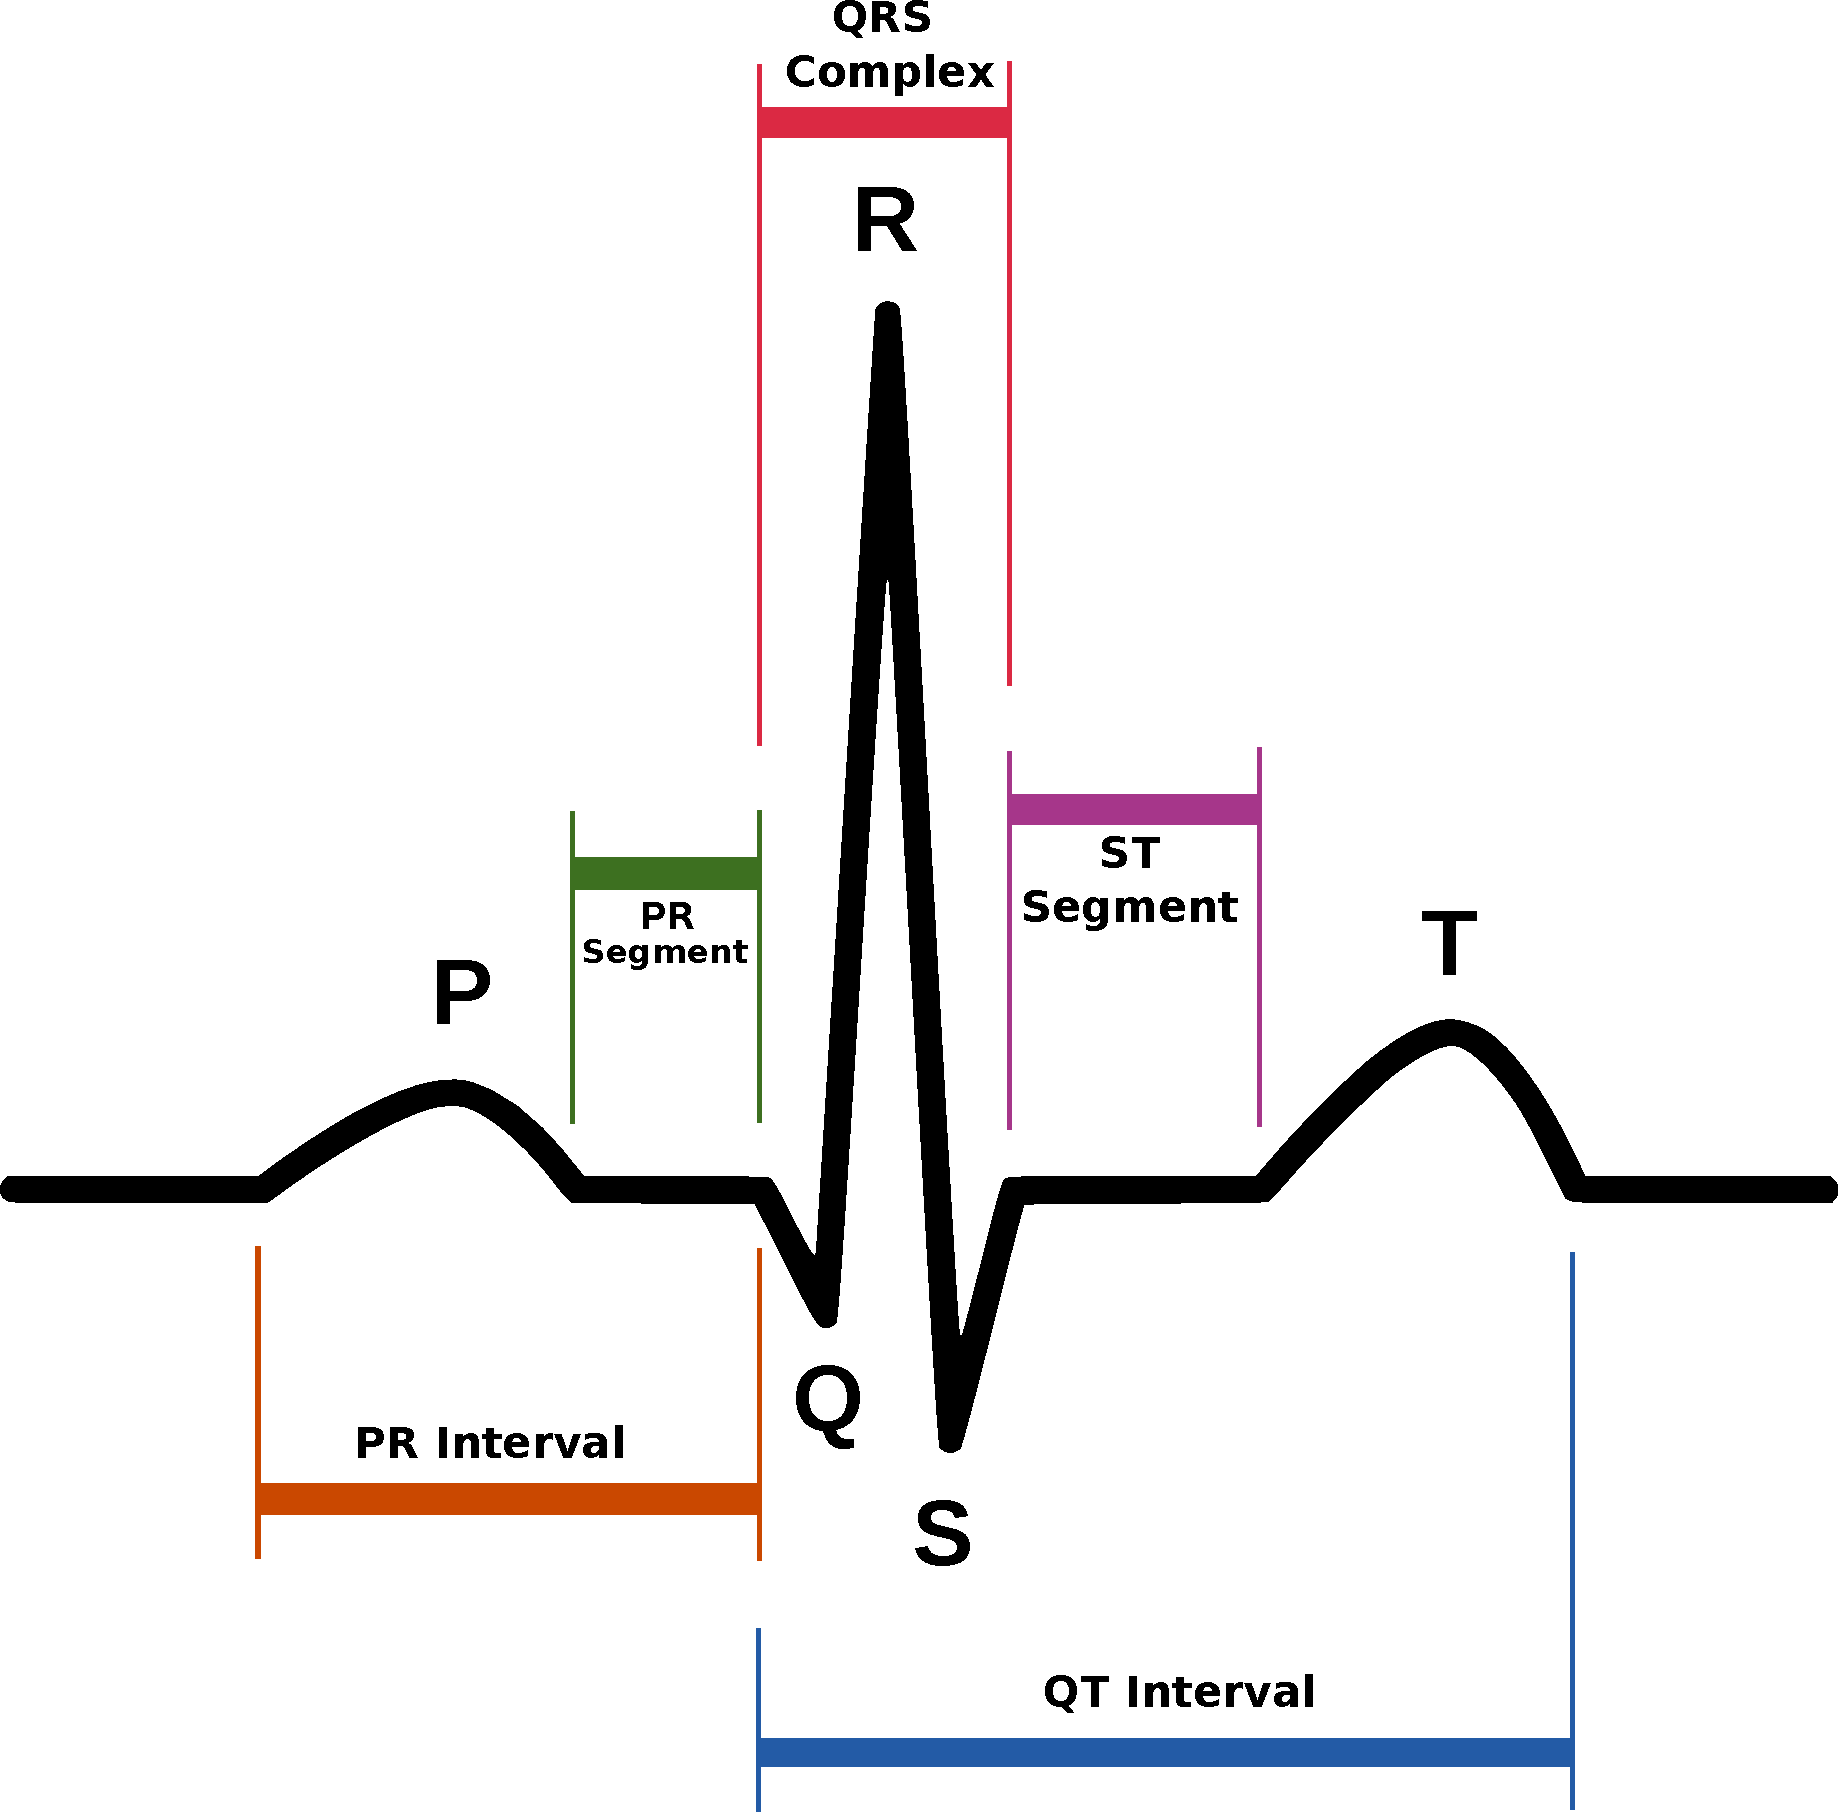
\includegraphics[width=0.5\textwidth]{figures/ecgFree.pdf}
\caption{\label{fig:ecg} Normal electrocardiogram.}
\end{center}
\end{figure} 
%%%%%%%%%%%%%%%%%%%%%%%%%%%%%%%%%%%%%%%%%%%%%%%%%%%%%%%%%%%%%%%%%%%%%%%%%%%%%%%%
%%%%%%%%%%%%%%%%%%%%%%%%%%%

The observable that is closest related to the action of the SA-node is the P 
wave and, thus,
the heartbeat period is defined as the time difference between two different P 
waves. However, the signal to noise ratio (SNR) 
of the P wave is smaller than the QRS complex SNR. Therefore, the QRS complexes 
are more
easily detected than the P waves and, for convenience, the heart beat period is 
computed as the time difference
between two successive QRS complexes. For the sake of simplicity, we will not 
discuss the QRS detectors in this tutorial.\\


\subsection{Constructing HRV time series}

After the QRS complex occurrences have been detected, the \gls{HRV} time series 
(sometimes called the RR time series) may be calculated.
The intervals between consecutive heart beats needed to construct the time 
series are called RR intervals, inter-beat intervals or interval function.
In some context, normal-to-normal intervals (NN) may also be used when 
referring to these intervals. \\

RR intervals are computed as the difference between successive R-wave 
occurrence times $t_n$. That is, the n-th RR interval 
$RR_n$ will be computed as 
\begin{equation}
RR_n=\alpha \cdot (t_n-t_{n-1}),
\label{Eq:RR}
\end{equation}
where $\alpha$ is a conversion parameter that may vary depending of the units 
in which the $RR$ time series is going to be expressed. Usually, the $RR$ 
intervals are expressed in ms and thus, if the occurrence times are expressed 
in seconds, $\alpha$ is setted as $\alpha=1000$.
It must be noticed that, in some studies, the \gls{HRV} is constructed as the 
sequence of the instantaneous
heart rates.  That is
\begin{equation}
\widehat{RR_n}=\frac{\beta}{t_n-t_{n-1}}.
\label{Eq:RRinst}
\end{equation}
Again, $\beta$ is used as a conversion parameter. Since the \gls{HR} is usually 
expressed in \gls{bpm},  $\beta=60$ if the occurrence times are expressed in 
seconds.
In this section, for the sake of simplicity, the $RR_n$ construction will be 
used.\\

The resulting RR series will consist of a set of pairs $(t_n,RR_n)$. It should 
be noted that this time series is not equidistantly sampled 
(that's why the time value, $t_n$, must be specified). This must be taken into 
account before frequency-domain analysis, since it requires an uniformly 
sampled time series. 
There are several approaches  to overcome this issue \cite{forceHRV}. RHRV  
uses interpolation for transforming the non-uniformly sampled RR series into an 
equidistantly sampled one. After interpolation, regular frequency analysis may 
be applied. A second approach, maybe the simplest one, assumes equidistant 
sampling and constructs a signal, called tachogram, using RR intervals as a 
function of a beat number. However, when using this approach, the spectrum is 
not a function of the frequency, rather of cycles per beat. A third approach 
receives the name
of the spectrum of the counts, that is, it uses a series of impulses (delta 
functions) 
positioned at beat occurrence times. This approach relies

on the commonly accepted Integral Pulse Frequency Modulator (IPFM) model 
\cite{berger1986},\cite{hyndman}, that simulates the modulation of the 
sinoatrial node.\\

%%%%%%%%%%%%%%%%%%%%%%%%%%%%%%%%%%%%%%%%%%%%%%%%%%%%%%%%%%%%%%%%%%%%%%%%%%%%%%%%
%%%%%%%%%%%%%%%%%%%%%%%%%%%
%\begin{figure}[ht]
%\begin{center}
%\includegraphics[scale=0.65]{figures/derivationHRV.pdf}
%\caption[Derivation of two HRV signals from an ECG record]{Derivation of two 
HRV signals from an ECG record: the left side of the figure shows
%a tachogram. The right side of the figure shows an interpolated \gls{HRV} 
signal and the Dirac deltas associated with each QRS complex. 
%This figure has been taken from \cite{kubios}.\label{fig:derivation}}
%\end{center}
%\end{figure} 
%%%%%%%%%%%%%%%%%%%%%%%%%%%%%%%%%%%%%%%%%%%%%%%%%%%%%%%%%%%%%%%%%%%%%%%%%%%%%%%%
%%%%%%%%%%%%%%%%%%%%%%%%%%%

\subsection{Preprocessing HRV time series}

Before performing the analysis of any RR time series, a filtering operation 
must be carried out in order to eliminate outliers or spurious points present 
in the signal with
unacceptable physiological values. Outliers present in the series originate 
from the detection of an artefact as a heartbeat (RR interval too short), or 
from the loss of a heartbeat in the detection procedure (RR interval too 
large). The RR time series may also contain some physiological artifacts. 
Physiological artefacts include ectopic beats (an ectopic beat occurs when the 
heart beat is not
triggered by the SA-node, causing an ``extra'' beat) and arrhythmic events. If 
detection of the heartbeat has been revised and corrected manually by a 
physician, this step can be skipped.\\

\section{HRV analysis techniques\label{sec:analysisTechn}}
The purpose of analysis techniques usually is to extract useful physiological 
information that may help  researchers to create new disease markers or 
predictors. There are several tools to perform \gls{HRV} analysis, however 
these are usually classified into three categories: time domain methods, 
frequency domain methods and non-linear methods. A brief review of the main 
techniques of time domain, frequency domain and nonlinear methods is presented. 
Further information may be found at \cite{forceHRV}.
\subsection{Time domain methods\label{sec:timedomain}}
The simplest \gls{HRV} analysis techniques are the time domain measures. Since 
there exist a wide variety of time domain techniques, we will focus on those 
included in the RHRV software. \\
The best known time analysis statistic may be the standard deviation of the RR 
interval: \gls{SDNN}.
$$SDNN=\sqrt{\frac{1}{N-1}\sum_{j=1}^{N}(RR_j-\overline{RR})^2}$$
Since the variance is mathematically equal to the total power of spectral 
analysis, \gls{SDNN} reflects the 
power of the components responsible for variability. The  \gls{SDNN} reflects 
both short-term and long-term variations within the RR  series. However, it 
should be noted that total variance of \gls{HRV}
increases with the length of the analysed recording \cite{saul1988analysis}. 
Thus, on arbitrarily ECGs,  \gls{SDNN}
may not be an appropriate \gls{HRV} analysis variable because of its dependence 
with the recording's length. To avoid this issue, statistical variables 
calculated from segments of the total monitoring period may be used. Among this 
kind of variables are the \glslink{SDANN}{SDANN}, the standard deviation of  
the average NN (RR) intervals calculated over short periods (usually 5 
minutes); and the \glslink{SDNNIDX}{SDNN index}, the mean
of the standard deviation calculated over the windowed RR intervals, usually 5 
minutes.\\

Other measures use the time series constructed as successive RR interval 
differences, defined as  $$\Delta RR_j=RR_{j+1}-RR_j.$$  The Root Mean square 
of Successive Differences (\glslink{RMSSD}{RMSSD}) is given by
$$RMSSD=\sqrt{\frac{1}{N-1}\sum_{j=1}^{N}(\Delta RR_j)^2}.$$

Other measures using the successive RR interval differences include the length 
of the interval determined by the first and the third quantile of the $\Delta 
RR$ time series; and the median of the absolute values of the  $\Delta RR$ time 
series (\glslink{MADRR}{MADRR}, Median of the Absolute Differences of the RR 
intervals).\\

Another commonly used measures derived from interval differences include NN50, 
the number of interval differences of successive RR intervals greater than 50 
ms, and \glslink{pNN50}{pNN50}, the proportion derived
by dividing NN50 by the total number of RR intervals.\\

All these measures derived from interval differences estimate the \gls{HF} 
variation in heart rhythm and thus, they are highly correlated.\\

Finally, in addition to these statistical parameters, there are some geometric 
measures that can be calculated from the RR interval histogram. The \gls{HRV} 
triangular index measurement is the integral of the density distribution (that 
is, the number of all RR intervals) divided by the maximum of the density 
distribution. The density distribution may be estimated by using an histogram, 
thus  the size of the bins should be specified. Another geometrical measure is 
the triangular interpolation of NN (RR) interval histogram 
(\glslink{TINN}{TINN}), which is calculated as the baseline width of the 
distribution measured as the base of a triangle (a triangular interpolation of 
the histogram may be used). The \glslink{TINN}{TINN} measure is usually 
expressed in milliseconds.\\

The major advantage of geometric methods lies in their relative insensitivity 
to the analytical quality of the RR series. Their major disadvantage is that 
they need a large number of RR intervals for performing
correctly.

\subsection{Frequency domain methods}
The basic frequency domain analysis technique  is the \gls{PSD}. It provides 
basic information on how power distributes as a function of frequency in the RR 
time series. Since the sympathetic an parasympathetic branches of the \gls{ANS} 
are associated with different frequency bands, the \gls{PSD} may be a useful 
tool to discriminate its different contributions to the \gls{HR}. The
most common approach to spectral analysis of \gls{HRV} is based on the Fourier 
transform. The Fourier transform is a tool that is able to extract the 
frequencies of a signal. For those unfamiliar with the ``frequency" language, 
we will say that a signal with fast and sharp changes has ``high frequencies", 
whereas a signal with slow transitions is referred to as a signal with ``low 
frequencies" (see Figure \ref{fig:sines}). Of course, a signal can contain both 
low and high frequencies. In this sense, the Fourier transform acts as a prism, 
separating the high frequency contributions from the low frequency 
contributions. The discrete implementation is referred to as the \gls{DFT} and 
its efficient implementation is called the \gls{FFT}.\\

The Fourier transform is one of the most powerful tools for signal processing. 
However, it may not be the most suitable tool for studying 
transient phenomena: the Fourier transform might be able to
determine all the frequencies present in a signal, but not when they are 
present. To address this issue, several techniques able to represent a signal 
in both time and frequency domain have been developed.\\

Following Gabor \cite{gabor1946}, the idea behind these time-frequency joint 
representations is to define elementary time-frequency atoms as
waveforms with minimum spread in the time-frequency plane. To measure 
time-frequency information content, Gabor proposed decomposing signals over 
these
elementary atoms. Selecting the time-frequency atoms is not a trivial problem 
because of the existence of a time-frequency uncertainty principle. This 
uncertainty principle states that the energy spread of a function and its 
Fourier transform  cannot  simultaneously be arbitrarily small.\\

The simplest transform that uses this idea is the windowed Fourier transform, 
that is  constructed by using a symmetric window that selects the portion of 
the signal that is going to be analyzed. The remaining portions of signal can 
be selected by translating the window in time. When this transform is applied 
to discrete signals, it is referred to as the \gls{STFT}.\\

\begin{figure}[h]
\centering
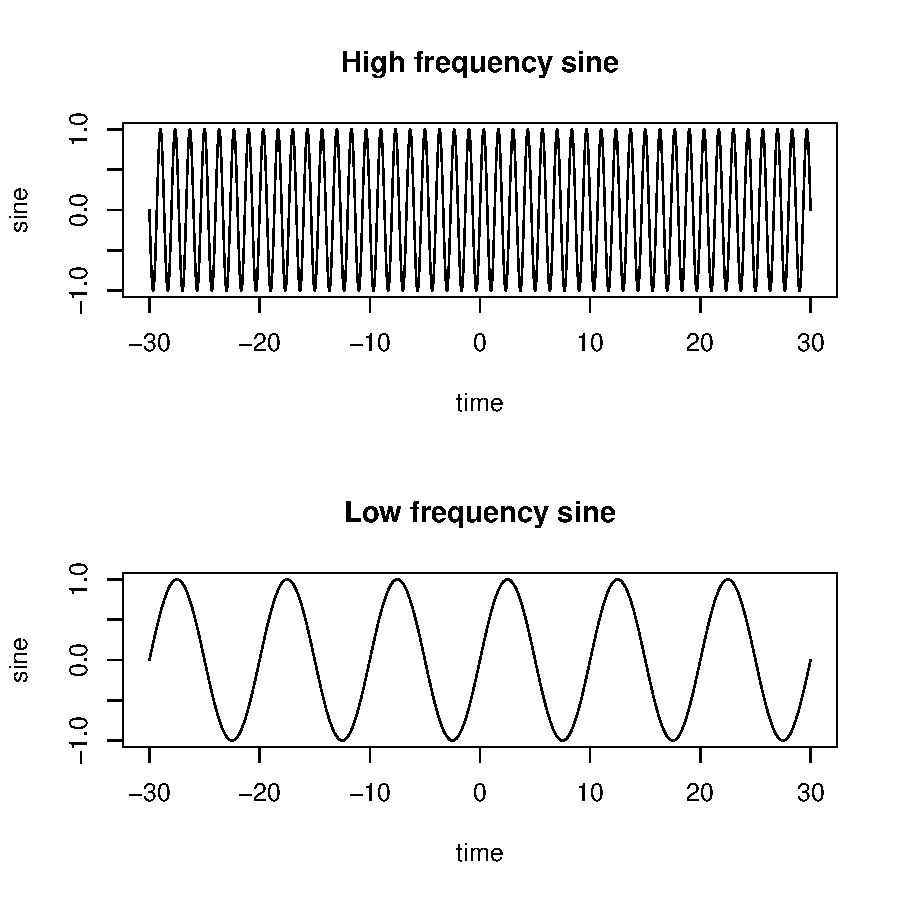
\includegraphics[width=0.6\textwidth]{figures/tutorial-highVslow}
\caption{High and low frequencies illustrated with sines.\label{fig:sines}}
\end{figure}

Another widely used transform that uses time-frequency atoms is the wavelet 
transform. A Wavelet is a ``small wave'' with zero mean that grows and decays 
in a limited time period. Since any of these small waves results in different 
wavelets, there are several wavelet families. Figure \ref{fig:wavelets} shows 
two such wavelets. The reference wavelet fulfilling the above conditions is 
called ``mother wavelet". The mother wavelet can be translated and dilated in 
time, yielding a set of wavelet functions with different sizes and centered in 
different time positions.  This set of functions is used to extract 
time-frequency information by correlating them with the signal being analyzed.\\

Although the idea of the wavelet transform is similar to that used in the 
\gls{STFT},  the wavelet transform often provides a better compromise between 
time and frequency resolution. This is due to the fact that the \gls{STFT} uses 
just one window for ``exploring" all the frequency bands. However, the ideal 
approximation would be using short windows at high frequencies and long windows 
at low frequencies. Thus, the ``global" performance of the \gls{STFT} will 
depend on the choice of the length of the window and the displacement time used 
for moving it. The wavelet transform, in contrast to the \gls{STFT}, follows 
the ideal approximation, leading to a multiresolution analysis. RHRV has 
support for both approaches, and they both have a similar computational 
efficiency.\\


%%%%%%%%%%%%%%%%%%%%%%%%%%%%%%%%%%%%%%%%%%%%%%%%%%%%%%%%%%%%%%%%%%%%%%%%%%%%%%%%
%%%%%%%%%%%%%%%%%%%%%%%%%%%
\begin{figure}[ht]
\begin{center}
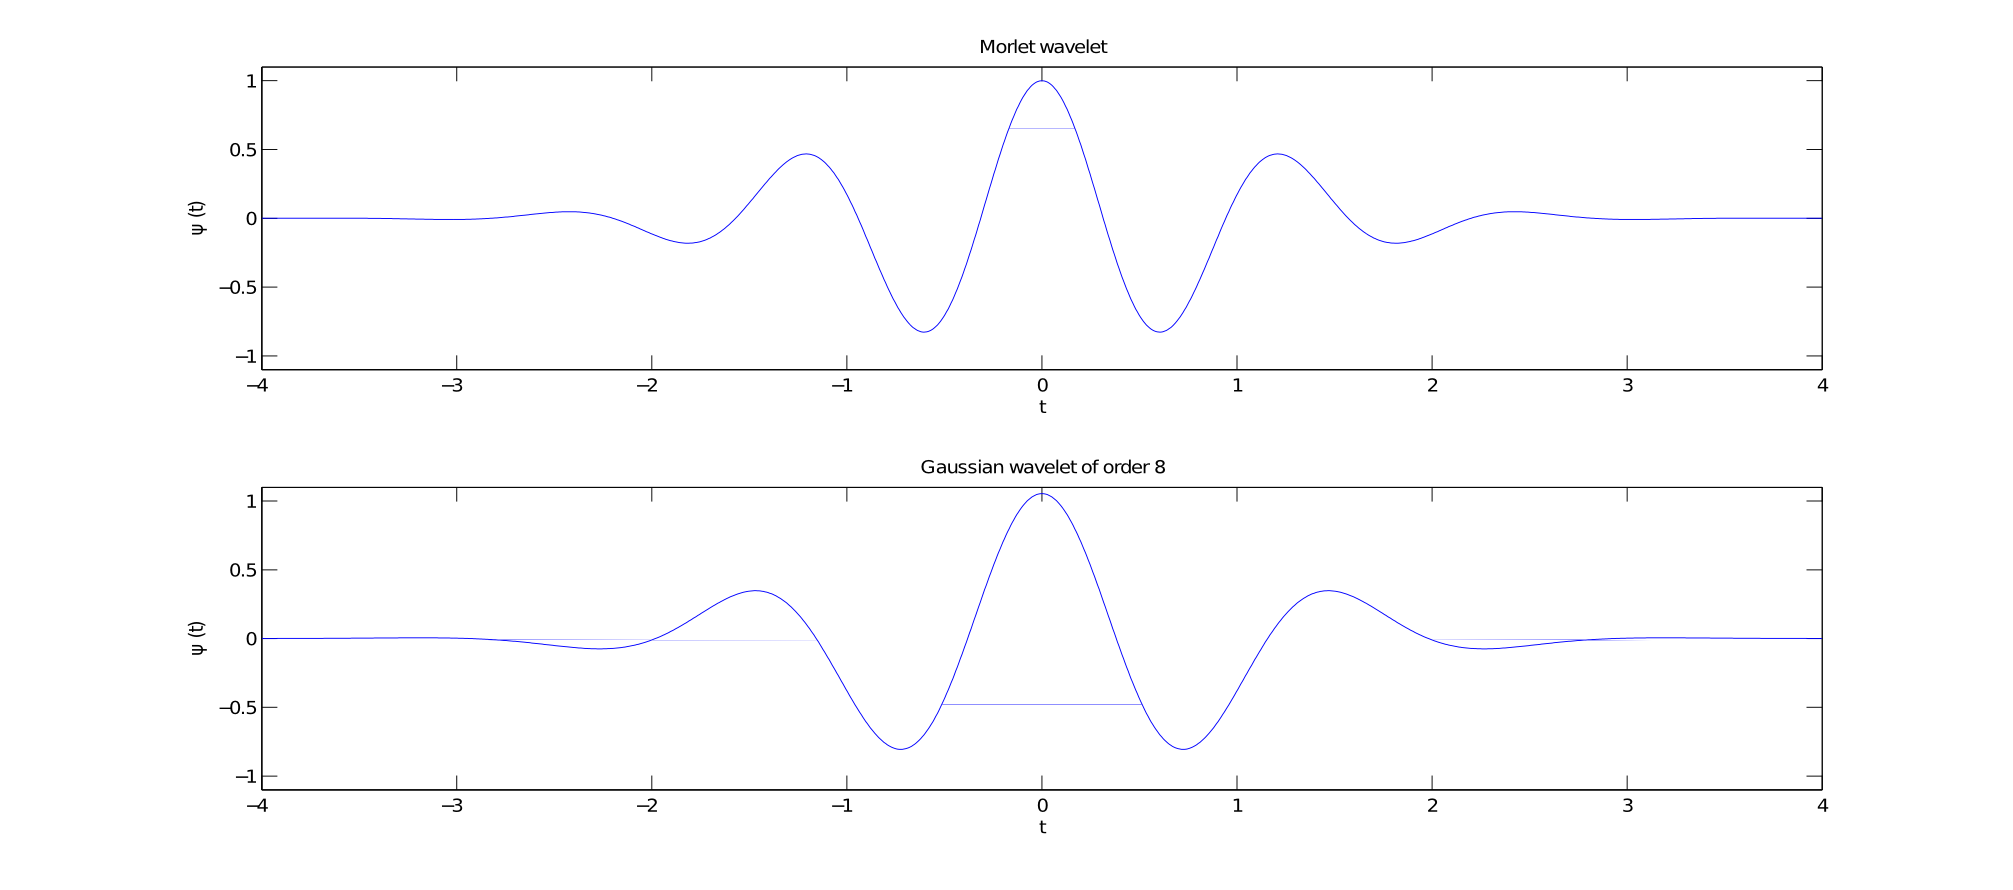
\includegraphics[scale=0.6]{figures/basicWavelets2.png}
\caption[Two Wavelets]{\label{fig:wavelets} Two Wavelets. The top of the figure 
shows the Morlet Wavelet. The bottom of the figure shows a Gaussian Wavelet.}
\end{center}
\end{figure} 
%%%%%%%%%%%%%%%%%%%%%%%%%%%%%%%%%%%%%%%%%%%%%%%%%%%%%%%%%%%%%%%%%%%%%%%%%%%%%%%%
%%%%%%%%%%%%%%%%%


When working with frequency methods, researchers are especially interested in 
the \gls{VLF}, \gls{LF} and \gls{HF} frequency bands. Some authors also include 
the \gls{ULF} band.
When selecting the frequency bands, the researchers should take into account 
whether they are working with short (2-5 min) or long term recordings (up to 
24-hours). Three main spectral components
are distinguished in a spectrum calculated from short-term recordings: 
\gls{VLF}, \gls{LF} and \gls{HF} components. However,  \gls{VLF} assessed from 
short-term recordings is 
a dubious  parameter and, therefore, it should be avoided when interpreting the 
\gls{PSD} in this kind of recordings \cite{forceHRV}. Spectral analysis 
resulting from long-term recordings include \gls{VLF}, \gls{LF} and \gls{HF} 
bands. In the long recordings, the \gls{VLF} band may be split into the 
\gls{ULF} and the \gls{VLF} components.\\

\subsection{nonlinear methods}
There is a profound connection between nonlinear phenomena and \gls{HRV}. 
\gls{HRV} is determined by complex interactions of electrophysiological and 
humoral variables, as well as by autonomic and central nervous regulations. 
Considering these complex control systems modulating the heart rhythm, it has 
been speculated that methods
of the nonlinear dynamics might extract some valuable information
from the \gls{HRV} series.\\

The measures that have been used to analyze nonlinear properties of \gls{HRV} 
include 1/f scaling of Fourier spectra, Poincar\'{e} plots, approximate and 
sample entropy, detrended fluctuation analysis, correlation dimension and 
recurrence plots. All these techniques have been shown to be powerful tools for 
extracting information from several complex systems, however, no really 
breakthrough results have yet been achieved when analyzing \gls{HRV} series.\\

Although there exist some functionality in the RHRV package for performing 
nonlinear analysis of a \gls{HR} signal it still is in ``beta". The current 
version of the tutorial will not treat these functions. Future versions of this 
tutorial will handle this issue.

\section{HRV alterations related to specific pathologies\label{sec:pathologies}}
In the course of the last two decades numerous studies have shown \gls{HRV} to 
be
a useful tool as a predictor of several pathologies such as myocardial 
infarction, sudden
cardiac death, heart failure, hypertension, and ischemia, among others 
\cite{malik1995}. 
However, it should be noted that the practical use of \gls{HRV} has reached
general consensus only in two clinical applications: as a predictor
of risk after myocardial infarction and as an early warning of diabetic 
neuropathy. \cite{forceHRV}, \cite{kautzner1997}.\\

Table \ref{t:diseases} resumes some \gls{HRV} applications to other diseases.\\

%\subsection{Myocardial infarction}
%
%Low \gls{HRV} after myocardial infarction (MI) reflects a decrease of the 
parasympathetic activity which leads
%to a prevalence of sympathetic mechanism on the heart rate. In the severe 
phase of MI,
% a reduction in 24-hours standard deviation of the \gls{HRV} signal has been 
registered. However, the mechanism by which \gls{HRV} is reduced
%after MI is not yet clear.\\
%
%Spectral analysis of \gls{HRV} in patients that suffered acute MI also reveals 
a reduction in total power and in each of the 
%power bands. When working with normalized units, an increase of the \gls{LF} 
and a diminished \gls{HF} activity is also observed.\\
%
%These characteristics of the spectral power distributions are also present in 
patients suffering from cardiac failure (in advanced
%state) and after cardiac transplant.\\
%
%The \gls{HRV} changes related to MI have led to the conclusion that a 
depressed \gls{HRV} is a powerful predictor of mortality and of arrhythmic
%complications in patients following acute MI. The value of both time-domain 
and frequency-domain parameters have been fully assessed in 
%several studies. It has also been proven that \gls{HRV} analysis is useful for 
risk stratification of patients following MI.\\
%
%\subsection{Diabetic neuropathy}
%
%As a complication of diabetes mellitus, autonomic neuropathy is characterized 
by early autonomic neuron degeneration,
% either parasympathetic or sympathetic, or both. Once clinical manifestation 
of diabetic autonomic neuropathy appear,
% the estimated 5-year mortality is approximately of 50\%. Thus, early 
predictive markers of autonomic dysfunction are important
% for risk stratification.\\
% 
%In neuropathy associated with diabetes mellitus, a reduction of time-domain 
parameters of \gls{HRV} 
%preceded the clinical detection of autonomic neuropathy.  In diabetic patients 
with no signs of 
%autonomic neuropathy, reduction of the absolute power in both \gls{LF} and 
\gls{HF} bands was also reported.
%However, when considering the LF/HF ratio no significant difference in 
comparison with normal patients was present.
%Thus, this means that the initial manifestation of this neuropathy involves 
both efferent limbs of the \gls{ANS}. All
%these abnormalities in \gls{HRV} analysis may be used as predictors of 
diabetic autonomic neuropathy occurrence.\\
%
%
%\subsection{Myocardial dysfunction}
%
%A reduced \gls{HRV} has been already observed in patients with cardiac 
failure. In fact, reduction in time domain measures
%of \gls{HRV} seemed to be more important with the severity of the disease. 
However, the relationship between spectral components
%and ventricular dysfunction  appears to be more complicated. In particular, in 
most patients suffering an advanced phase of the disease
%and with drastic reduction in \gls{HRV}, a \gls{LF} component could not be 
detected despite clinical signs of sympathetic activation (such as 
%faster heart rates). Thus, SA-node seems to diminish its responsiveness to 
\gls{ANS} modulation.\\



%%%%%%%%%%%%%%%%%%%%%%%%%%%%%%%%%%%%%%%%%%%%%%%%%%%%%%%%%%%%%%%%%%%%
\begin{center}
\scriptsize
\begin{longtable}{|p{4cm}|p{4cm}|p{4cm}|}
\caption[Clinical value of HRV analysis in cardiological diseases]
{Summary of the clinical value of HRV analysis in cardiological diseases. Inspired by \cite{forceHRV}.} \label{t:diseases} \\

\hline \multicolumn{1}{|c|}{\textbf{Disease state}} & \multicolumn{1}{c|}{\textbf{Clinical finding }} & \multicolumn{1}{c|}{\textbf{Potential value}} \\ \hline 
\endfirsthead

\multicolumn{3}{c}%
{{\bfseries \tablename\ \thetable{} -- continued from previous page}} \\
\hline \multicolumn{1}{|c|}{\textbf{Disease state}} &
\multicolumn{1}{c|}{\textbf{Clinical findings}} &
\multicolumn{1}{c|}{\textbf{Potential value}} \\ \hline 
\endhead

\hline \multicolumn{3}{|c|}{{Continued on next page}} \\ \hline
\endfoot

\hline \hline
\endlastfoot
Myocardial infarction (MI)&$\downarrow$ HRV after myocardial infarction (MI). In the severe phase of MI, there is a $\downarrow$ standard deviation of the HRV signal& Depressed HRV is a powerful predictor of mortality and of arrhythmic
complications in patients following acute MI\\ \cline{3-3}
& &HRV analysis is useful for risk stratification of patients following MI\\ \hline

Diabetic neuropathy& $\downarrow$ time-domain parameters of HRV 
preceded the clinical detection of autonomic neuropathy. $\downarrow$ LF and HF bands  in diabetic patients with no signs of 
autonomic neuropathy& HRV analysis may be used as predictor of diabetic autonomic neuropathy occurrence\\ \hline
Hypertension&$\uparrow$ LF found in hypertensives with circadian patterns& Hypertension is characterized by depressed circadian rhythmicity of LF\\ \cline{2-3}
            &Reduced parasympathetic activity in hypertensive patients&\\ \hline
Congestive heart failure (CHF)&$\downarrow$ spectral power in all frequencies, especially $>0.04$ Hz&In CHF, there is $\downarrow$ vagal, but relatively
preserved sympathetic modulation of HR\\ \cline{2-3}
		&Low HRV&Reduced vagal activity in CHF patients\\ \cline{2-3}
		&$\downarrow$ HF power in CHF.$\uparrow$ LF/HF& Low parasympathetic tone in CHF. CHF produces imbalance of autonomic tone with $\downarrow$ parasympathetic and predominance of sympathetic tone\\\cline{2-3}
		&Alterations in HRV not tightly linked to severity of CHF. $\downarrow$ HRV was related to sympathetic excitation& \\ \cline{2-3}
		&$\uparrow$ HRV during ACE (angiotensin-converting-enzyme) inhibitor treatment&Increase of the sympathetic tone associated with ACE inhibitor therapy\\ \hline
Heart Transplantation&HRV from $0.02$ to $1$ Hz is $90\%$ reduced& Patients with rejection show less variability\\ \hline
Chronic mitral regurgitation&HR techniques correlated with ventricular performance and predicted clinical events&Prognostic indicator of atrial fibrillation, mortality and progression to valve surgery\\ \hline
Mitral Valve prolapse (MVP)&$\downarrow$ HF power&MVP patients had low vagal tone\\ \hline
Cardiomyopathies&Global and specific vagal tone measurements of HRV were $\downarrow$ in symptomatic patients&\\ \hline
Sudden death (SD) or cardiac arrest (CA)&LF power and standard deviation of HRV signals were related to 1 year mortality&HRV is useful to risk stratify CA survivors for 1 year mortality\\ \cline{2-3}
	&$\downarrow$ HF power in CA survivors&\\ \cline{2-3}
	&Both time and frequency domain indexes separated controls from SD patients. $\downarrow$ HF power was the best separator between heart disease patients
	with and without SD& HF power may be useful predictor of SD\\\cline{2-3}
	&SDNN index was lower in SD patients&Time domain indexes may identify increased risk of SD\\ \hline
Ventricular arrhythmias&HRV indexes do not change consistently before ventricular fibrillation (VF). All power spectra of HRV were significantly $\downarrow$ before the onset of sustained ventricular tachycardia (VT) than before non sustained VT & A temporal relation exists between the decrease of HRV and the onset of sustained VT \\ \hline
\end{longtable}
\end{center}


%%%%%%%%%%%%%%%%%%%%%%%%%%%%%%%%%%%%%%%%%%%%%%%%%%%%%%%%%%%%%%%%%%%%%


%%%%% New chapter %%%%%%
% !Rnw root = ../../tutorial.Rnw
\chapter{Installation\label{ch:installation}}
\section{Installation} This guide assumes that the user has some basic 
knowledge of the R environment. If this is not your case, you can find a nice 
introduction to R in the R project homepage \cite{Rproject}. The R project 
homepage also provides an ``R Installation and Administration" guide. Once you 
have download and installed R, you can install RHRV by typing:
\begin{Schunk}
\begin{Sinput}
> install.packages("RHRV")
\end{Sinput}
\end{Schunk}
You can also install it by downloading it from the CRAN \cite{cran}. Once the 
download has finished, open R , move to the directory where you have download 
it (by using the R command \textit{setwd}) and type:

\begin{Schunk}
\begin{Sinput}
> install.packages("RHRV_XXX",repos=NULL)
\end{Sinput}
\end{Schunk}
Here, XXX is the version number of the library. To start using the library, you 
should load it by using the \textit{library} command:
\begin{Schunk}
\begin{Sinput}
> library(RHRV)
\end{Sinput}
\end{Schunk}

\section{WFDB applications} Some functions of the RHRV package (such as the 
\textit{LoadApneaWFDB}) require the installation of the WFDB functions 
\cite{moody2003wfdb}. If the user is not going to work with WFDB formated 
files, the installation of these libraries is not required for the proper 
functioning of RHRV. The WFDB functions is a large collection of specialized 
software for processing and manipulating the Physionet's databases 
\cite{physioNet}. On Windows and Mac OSX operating systems is necessary to 
define
a .Renviron file in the user workspace indicating the directory
of the WFDB commands. Examples for both OS are given below: 
\begin{verbatim}
## .Renviron on Windows
PATH = "c:\\cygwin\\bin"
DYLD_LIBRARY_PATH = "c:\\cygwin\\lib"
\end{verbatim}

\begin{verbatim}
## .Renviron on Macosx
PATH = "/opt/local/bin"
DYLD_LIBRARY_PATH = "/opt/local/bin"
\end{verbatim}


\section{Troubleshooting} 
\subsection[tkrplot dependency]{When installing the RHRV package in linux, 
sometimes the installation fails when installing the tkrplot dependency.}
\begin{verbatim}
...
tcltkimg.c:2:16: fatal error: tk.h: No such file or directory
compilation terminated.

ERROR: compilation failed for package 'tkrplot'
...
ERROR: dependency 'tkrplot' is not available for package 'RHRV'
\end{verbatim}

This is usually because there are some missing libraries in your system. 
Generally, the problem will be fixed by installing the \textit{tclX.X}, 
\textit{tkX.X}, \textit{tclX.X-dev} and  \textit{tkX.X-dev} libraries (X.X 
stands for the version of the libraries). 


%%%%% New chapter %%%%%%
% !Rnw root = ../../tutorial.Rnw
\chapter{A 15-minutes guide to RHRV\label{ch:Quick}}
% !Rnw root = ../15guide.Rnw
In this chapter, a brief description of the RHRV package is presented 
\cite{vilaRHRV}. Due to the large collection of features that RHRV offers, in 
this chapter we shall refer only to the most important functionality for 
performing  a basic \gls{HRV} analysis. In the next chapter we will present 
more advanced functionality of the package, or functionality geared to certain 
particular types of analysis. RHRV can be freely downloaded from the R-CRAN 
repository \cite{cran}.\\

We propose the following basic program flow to perform \gls{HRV} spectral 
analysis using the RHRV package:

\begin{enumerate}
\item Load heart beat positions. For the sake of simplicity, in this section we 
will focus in
ASCII files. 
\item Build the instantaneous \gls{HR} series and filter it to eliminate 
spurious points.
\item Plot the instantaneous \gls{HR} series.
\item Interpolate the instantaneous \gls{HR} series to obtain a \gls{HR} series 
with equally spaced values.
\item Plot the interpolated \gls{HR} series.
\item Perform the desired analysis. The user can perform time-domain analysis, 
frequency-domain analysis or nonlinear analysis.
\item Plot the results of the analysis that has been performed and access the 
``raw" data.
\end{enumerate}
In section \ref{sec:quickPrep} we will address points 1-5, whereas that in 
section \ref{sec:quickAna} we will deal with points 6 and 7. All the examples 
of this chapter will use the 
example beats file ``example.beats" that may be downloaded from 
\href{http://rhrv.r-forge.r-project.org/}{http://rhrv.r-forge.r-project.org/}. 
Optionally, the data from this file has been included in RHRV. The user can 
access this data executing:

\begin{Schunk}
\begin{Sinput}
> # HRVData structure containing the heart beats 
> data("HRVData")
> # HRVData structure storing the results of processing the 
> # heart beats: the beats have been filtered, interpolated, ... 
> data("HRVProcessedData")
\end{Sinput}
\end{Schunk}
The example file is an ASCII file that contains the beats positions obtained 
from a 2 hours \gls{ECG} (one beat position per row). The subject of the 
\gls{ECG} is a patient suffering from paraplegia and hypertension (systolic 
blood pressure above 200 mmHg).  During the recording, he is supplied with 
prostaglandin E1 (a vasodilator that is rarely employed) and systolic blood 
pressure fell to 100 mmHg for over an hour. Then, the blood pressure increased 
slowly up to approximately
 150 mmHg. 

The console output shall be shown for every example.
\section{Preprocessing the Heart Rate series\label{sec:quickPrep}}
% !Rnw root = ../15guide.Rnw
\subsubsection{Load heart beat positions} RHRV uses a custom data structure 
called \textit{HRVData} to store all HRV information related to the signal 
being analyzed. \textit{HRVData} is implemented as a list object in R language. 
This list contains all the information corresponding
to the imported signal to be analyzed, some parameters generated
by the pre-processing functions and the HRV analysis results.  A new 
\textit{HRVData} structure is created using the \textit{CreateHRVData} 
function. In order to obtain detailed information about
the operations performed by the program, we can activate a verbose mode using 
the \textit{SetVerbose} function.
\begin{Schunk}
\begin{Sinput}
> hrv.data  = CreateHRVData()
> hrv.data = SetVerbose(hrv.data, TRUE )
\end{Sinput}
\end{Schunk}

After creating the empty \textit{HRVData} structure  the next step should be 
loading the signal that we want to analyze into this structure. RHRV imports 
data files containing heart beats positions. Supported formats include ASCII 
(\textit{LoadBeatAscii} function), EDF (\textit{LoadBeatEDFPlus}), Polar 
(\textit{LoadBeatPolar}), Suunto (\textit{LoadBeatSuunto}) and WFDB data files 
(\textit{LoadBeatWFDB}) \cite{mitbih}. For the sake of simplicity, we will 
focus in
ASCII files containing one heart beat occurrence time per line. We also assume 
that the beat occurrence time is specified in seconds (further details will be 
given in chapter \ref{ch:RHRV}). For example, let's try to load the 
``example.beats" file, whose first lines are shown below. Each line denotes
the occurrence time of each heartbeat.
\begin{verbatim}
0
0.3280001
0.7159996
1.124
1.5
1.88
\end{verbatim}
In order to load this file, we may write:
\begin{Schunk}
\begin{Sinput}
> hrv.data = LoadBeatAscii(hrv.data, "example.beats",
+        RecordPath = "beatsFolder")
\end{Sinput}
\begin{Soutput}
** Loading beats positions for record: example.beats **
   Path: beatsFolder 
   Scale: 1 
   Date: 01/01/1900
   Time: 00:00:00
   Number of beats: 17360 
\end{Soutput}
\end{Schunk}
The console information is only displayed if the verbose mode is on. The
\textit{Scale} parameter is related to the time units of the file. $1$
denotes seconds, $0.1$ deciseconds and so on. The \textit{Date} and 
\textit{Time}
parameters specify when the file was recorded. More details about these
parameters will be given in section \ref{sec:moreReading}. The 
\textit{RecordPath} can be omitted if the \textit{RecordName} is in the 
working directory.
\subsubsection{Calculating HR and filtering} To compute the HRV time series the 
\textit{BuildNIHR} function can be used (\textit{Build Non Interpolated Heart 
Rate}). This function constructs both the RR (Equation \ref{Eq:RR}) and 
instantaneous heart rate (\gls{HR}) series (Equation \ref{Eq:RRinst}) described 
in Section \ref{sec:obtainingHRV}. We will refer to the instantaneous heart 
rate (\gls{HR}) as the 
\gls{niHR} series. Both series are stored in the \textit{HRVData} structure.\\

\begin{Schunk}
\begin{Sinput}
> hrv.data = BuildNIHR(hrv.data)
\end{Sinput}
\begin{Soutput}
** Calculating non-interpolated heart rate **
   Number of beats: 17360 
\end{Soutput}
\end{Schunk}

A Filtering operation must be carried out in order to eliminate outliers or 
spurious points present in the \gls{niHR} time series with
unacceptable physiological values. Outliers present in the series originate 
from the detection of an artefact as a heartbeat (RR interval too short) and 
loss of a heartbeat in the detection procedure (RR interval too large). The 
outliers removal may be both manual or automatic. In this quick introduction, 
we will use the automatic removal.  The automatic removal of spurious points 
can be performed by the \textit{FilterNIHR} function. The \textit{FilterNIHR} 
function also eliminates points with unacceptable physiological values.\\
\begin{Schunk}
\begin{Sinput}
> hrv.data = FilterNIHR(hrv.data)
\end{Sinput}
\begin{Soutput}
** Filtering non-interpolated Heart Rate **
   Number of original beats: 17360 
   Number of accepted beats: 17178 
\end{Soutput}
\end{Schunk}
\subsubsection{Interpolating} In order to be able to perform spectral analysis 
in the frequency domain, a uniformly sampled \gls{HR} series is required. It 
may be constructed from the \gls{niHR} series by using the 
\textit{InterpolateNIHR} function, which uses linear (default) or spline 
interpolation  (further details
on chapter \ref{ch:RHRV}). The frequency of interpolation may be specified. 
$4\;Hz $ (the default value) is  enough for most applications.

\begin{Schunk}
\begin{Sinput}
> # Note that it is not necessary to specify freqhr since it matches with
> # the default value: 4 Hz
> hrv.data = InterpolateNIHR (hrv.data, freqhr = 4)
\end{Sinput}
\begin{Soutput}
** Interpolating instantaneous heart rate **
   Frequency: 4Hz
   Number of beats: 17178 
   Number of points: 29594 
\end{Soutput}
\end{Schunk}

\subsubsection{Plotting} Before applying the different analysis techniques that 
RHRV provides, it 
is usually interesting to plot the time series with which we are working. The 
\textit{PlotNIHR} function permits the graphical representation of the 
\gls{niHR} series whereas that the \textit{PlotHR} function permits to 
graphically represent the interpolated \gls{HR} time series.\\
\begin{Schunk}
\begin{Sinput}
> PlotNIHR(hrv.data)
\end{Sinput}
\end{Schunk}
\begin{Schunk}
\begin{Sinput}
> PlotHR(hrv.data)
\end{Sinput}
\end{Schunk}
The plots obtained with \textit{PlotNIHR} and \textit{PlotHR} are shown in 
Figures \ref{fig:exampleNIHR} and \ref{fig:exampleHR}, respectively.\\

\begin{figure}[h]
\centering
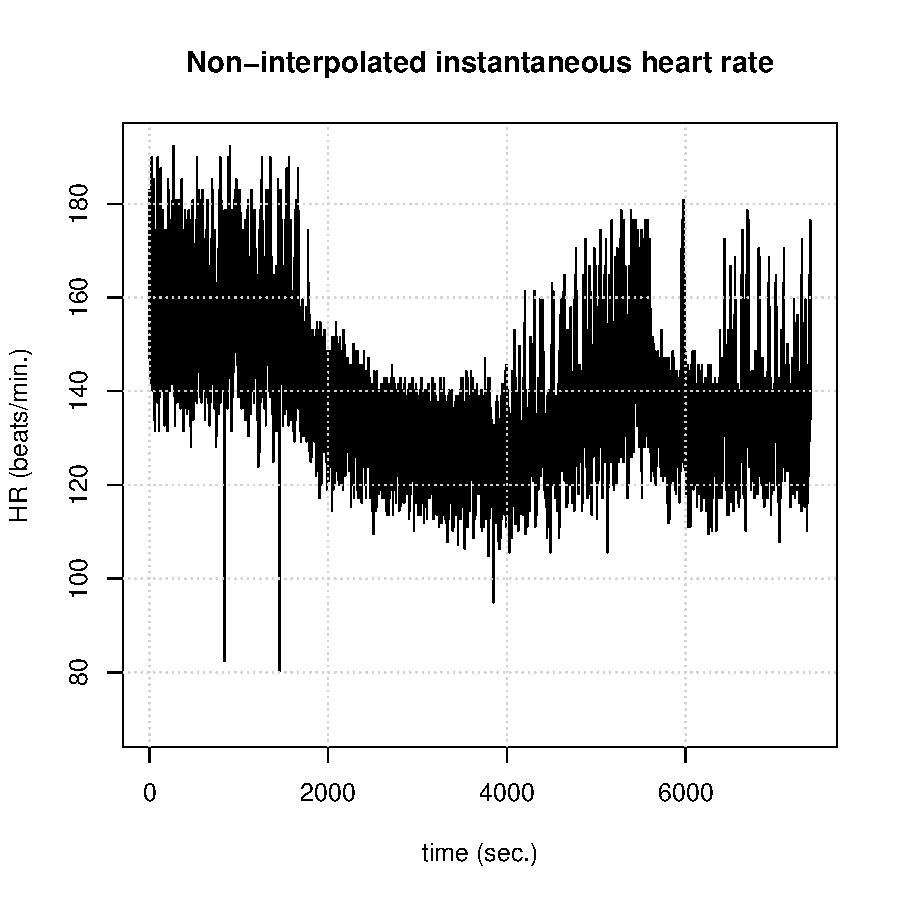
\includegraphics{figures/tutorial-plottingNIHR}
\caption{Non interpolated Heart Rate time plot example.\label{fig:exampleNIHR}}
\end{figure}

\begin{figure}[h]
\centering
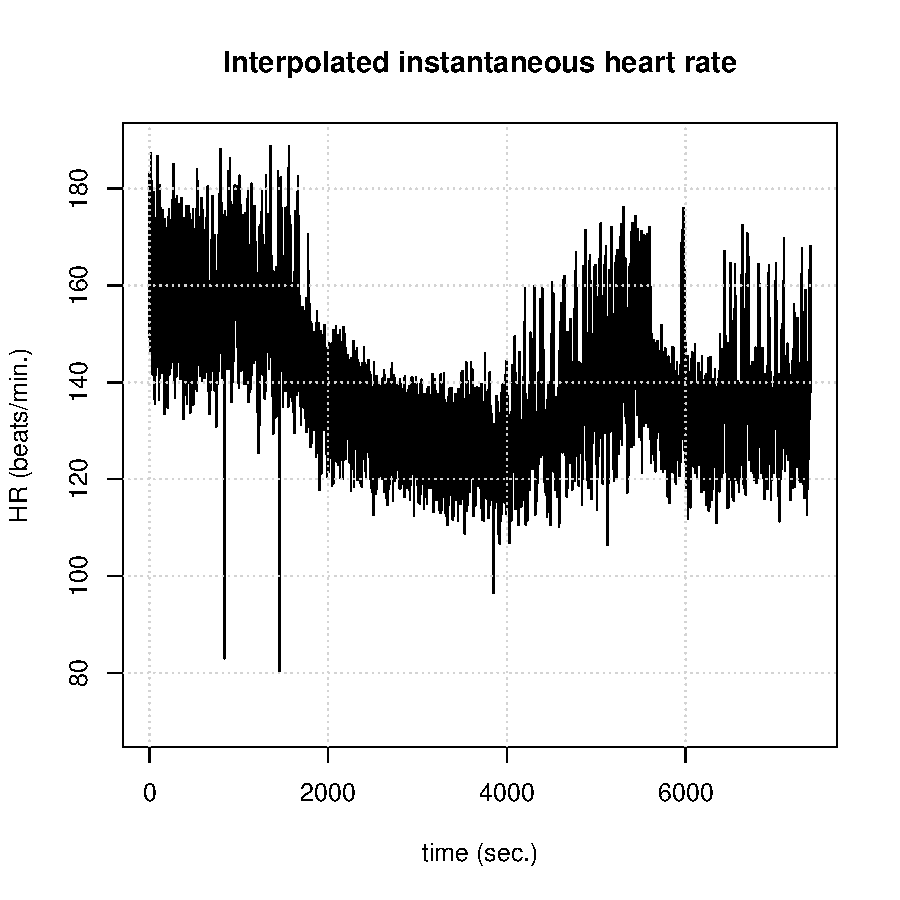
\includegraphics{figures/tutorial-plottingHR}
\caption{Interpolated Heart Rate time plot example.\label{fig:exampleHR}}
\end{figure}

As seen in the Figures \ref{fig:exampleNIHR} and \ref{fig:exampleHR}, the 
patient initially had a heart rate of approximately 160 beats per minute. 
Approximately half an hour into record the prostaglandina E1 was provided, 
resulting in a drop in heart rate to about 130 beats per minute during about 40 
minutes, followed by a slightt increae in heart rate.
\section{Analysing the Heart Rate series\label{sec:quickAna}}
% !Rnw root = ../../15guide.Rnw
\subsection{Accessing ``raw data"}
% !Rnw root = analyzing.Rnw
In the previous sections, we have used the 
\textit{HRVData}  structure  to store all \gls{HRV} information related to the 
signal being analyzed with no knowledge about its internal structure. However, 
sometimes, in order to make some particular analysis of the data, it may be 
interesting to access them directly. Figure \ref{fig:dataScheme} summarizes the 
most important fields in the
\textit{HRVData} structure. Since all the data in this structure is stored as 
an R list, each of its fields can be accessed using the \$ operator of the R 
language. For example, if we want to access the RR time series of the 
\textit{hrv.data}, we would use:
\begin{Schunk}
\begin{Sinput}
> RR = hrv.data$Beat$RR
\end{Sinput}
\end{Schunk}

\begin{figure}[h]
\centering
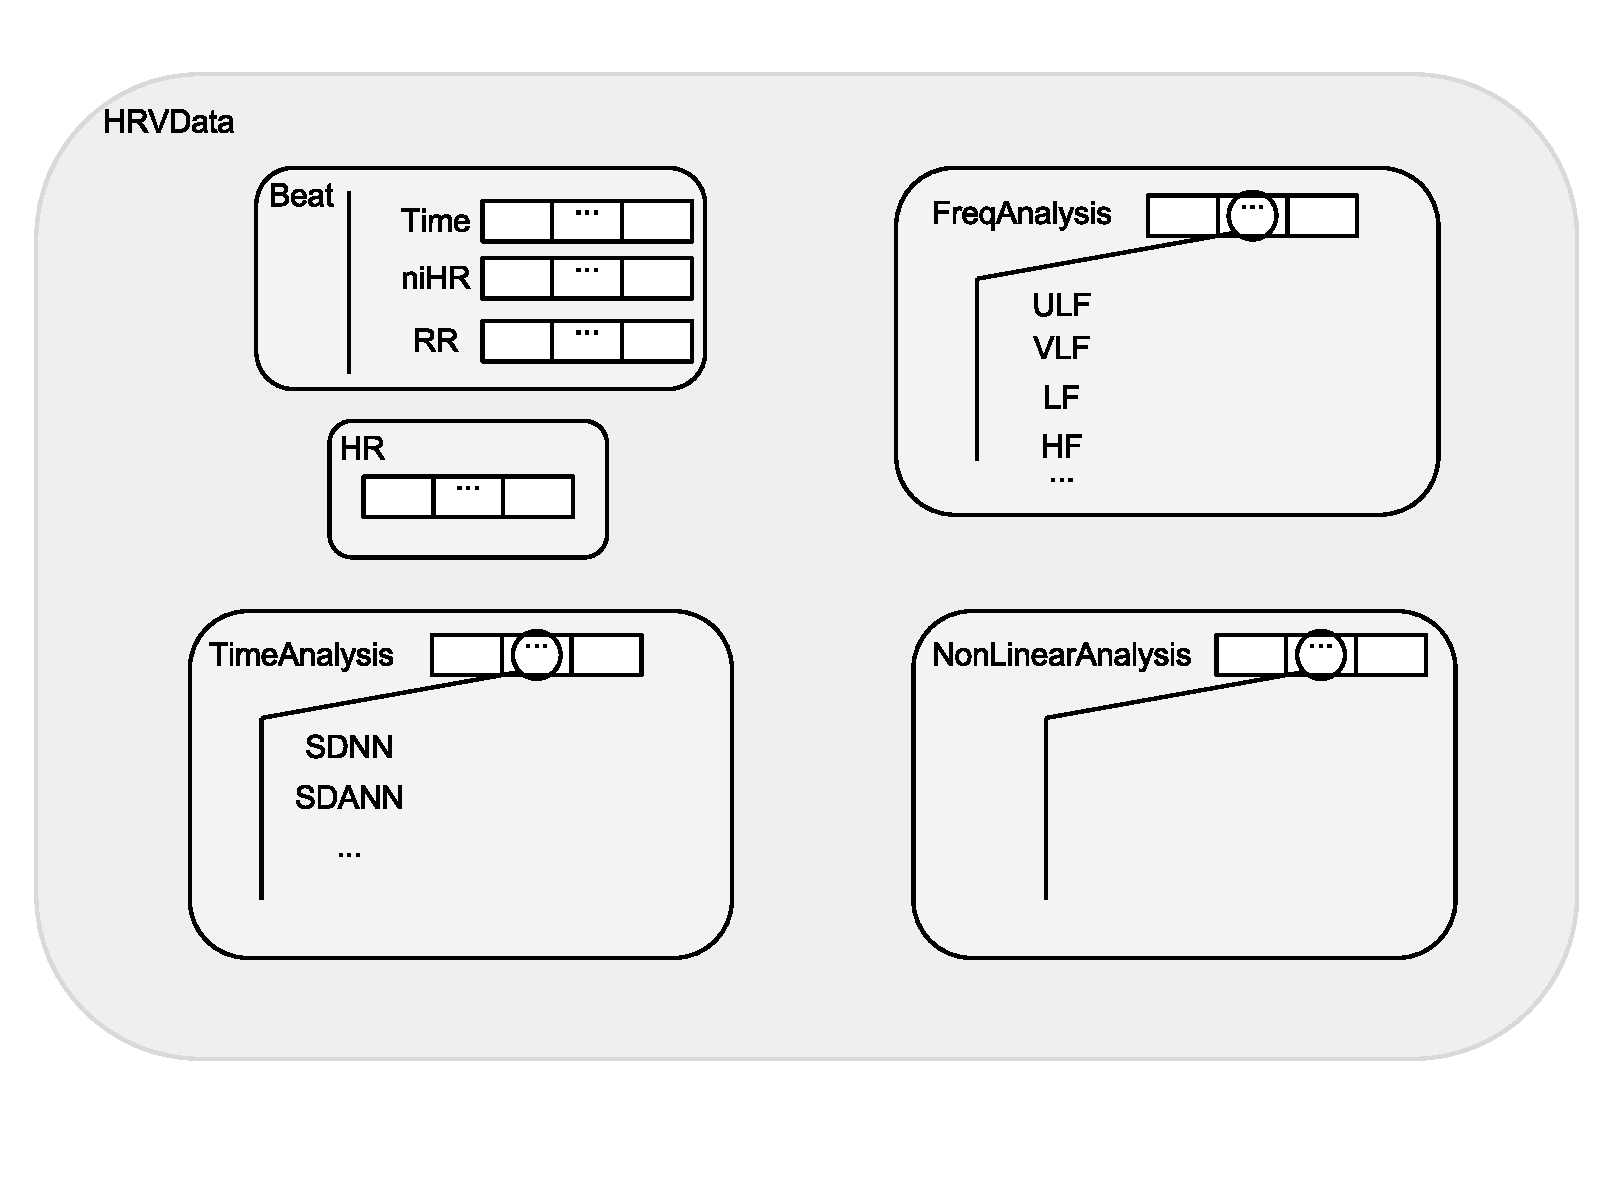
\includegraphics{figures/basicHRVData.pdf}
\caption{The most important fields stored in the \textit{HRVData} 
structure.\label{fig:dataScheme}}
\end{figure}
Although it is an advantage to be familiarized with the \textit{HRVData} 
structure, there is no need to memorize it since we can use the useful 
\textit{name} R function. Thus, if we want to know which fields are stored into 
the \textit{hrv.data\$Beat} subfield, we could use:

\begin{Schunk}
\begin{Sinput}
> names(hrv.data$Beat)
\end{Sinput}
\begin{Soutput}
[1] "Time" "niHR" "RR"  
\end{Soutput}
\end{Schunk}

As we can see,  \textit{hrv.data\$Beat} stores the occurrence time of each beat 
(\textit{``Time"}), the \gls{niHR} time series (\textit{``niHR"}) and the RR 
time series (\textit{``RR"}).
\subsection{Time-domain analysis techniques\label{sec:quickTime}}
% !Rnw root = analyzing.Rnw
The simplest way of performing a \gls{HRV} analysis in RHRV is using the time 
analysis techniques 
provided by the \textit{CreateTimeAnalysis} function. This function computes 
the time-domain
parameters presented in section \ref{sec:timedomain} and stores them in the 
\textit{HRVData} structure. The most interesting parameter that the user may 
specify is the width of the window that
will be used to analyze short segments from the RR time series (\textit{size} 
parameter, in seconds). Concretely, several statistics will be computed for 
each window. By studying how these statistics
evolve through the recording, a set of time parameters will be computed (For 
example, the \textit{SDANN}
and \textit{SDNNIDX} parameters). Other important argument that can be tuned is 
the interval width of the bins that will be used to compute the histogram 
(\textit{interval} parameter). As an alternative to the \textit{interval} 
parameter, the user may use the 
\textit{numofbins} parameter to specify the number of bins in the histogram. A 
typical value for the \textit{size} parameter is 300 seconds (which is also the 
default value), whereas that a typical value for the \textit{interval} is about 
7.8 milliseconds (also default value).

\begin{Schunk}
\begin{Sinput}
> hrv.data = CreateTimeAnalysis(hrv.data, size = 300,
+     		interval = 7.8125)
\end{Sinput}
\begin{Soutput}
** Creating time analysis
   Size of window: 300 seconds 
   Width of bins in histogram: 7.8125 milliseconds 
   Number of windows: 24 
   Data has now 1 time analyses
      SDNN: 39.34843 msec. 
      SDANN: 31.05912 msec. 
      SDNNIDX: 24.46209 msec. 
      pNN50: 8.63946 %
      SDSD: 29.92308 msec.
      r-MSSD: 29.92221 msec.
      IRRR: 32 msec.
      MADRR: 16 msec.
      TINN: 86.80668 msec.
      HRV index: 11.11125 
\end{Soutput}
\end{Schunk}
If the verbose mode is on, the program will display the results of the 
calculations in the screen. Otherwise, the user must access the ``raw" data as 
explained before to obtain the results.\\

Finally, we show a complete example for performing a basic time-domain 
analysis. The console output is also shown. It should be noted that it is not 
necessary to perform the interpolation process before applying 
the time-domain techniques since these parameters are calculated directly from 
the RR-time series. \\
\begin{Schunk}
\begin{Sinput}
> hrv.data = CreateHRVData()
> hrv.data = SetVerbose(hrv.data,FALSE)
> hrv.data = LoadBeatAscii(hrv.data,"example.beats","beatsFolder")
> hrv.data = BuildNIHR(hrv.data)
> hrv.data = FilterNIHR(hrv.data)
> PlotNIHR(hrv.data)
> hrv.data = SetVerbose(hrv.data,TRUE)
> hrv.data = CreateTimeAnalysis(hrv.data,size=300,interval = 7.8125)
\end{Sinput}
\begin{Soutput}
** Creating time analysis
   Size of window: 300 seconds 
   Width of bins in histogram: 7.8125 milliseconds 
   Number of windows: 24 
   Data has now 1 time analyses
      SDNN: 39.34843 msec. 
      SDANN: 31.05912 msec. 
      SDNNIDX: 24.46209 msec. 
      pNN50: 8.63946 %
      SDSD: 29.92308 msec.
      r-MSSD: 29.92221 msec.
      IRRR: 32 msec.
      MADRR: 16 msec.
      TINN: 86.80668 msec.
      HRV index: 11.11125 
\end{Soutput}
\begin{Sinput}
> # We can access "raw" data... let's print separately, the SDNN 
> # parameter
> cat("The SDNN has a value of ",hrv.data$TimeAnalysis[[1]]$SDNN," msec.\n")
\end{Sinput}
\begin{Soutput}
The SDNN has a value of  39.34843  msec.
\end{Soutput}
\end{Schunk}

\subsection{Frequency-domain analysis techniques\label{sec:quickFreq}}
% !Rnw root = analyzing.Rnw
A major part of the functionality of the RHRV package is dedicated to the 
spectral analysis of \gls{HR} signals. Before performing the frequency 
analysis, a data analysis structure must be created. Such structure shall store 
the information extracted from a variability analysis of the \gls{HR} signal as 
a member of the \textit{FreqAnalysis} list, under the \textit{HRVData} 
structure. Each analysis structure created is identified by a unique number (in 
order of creation). To create such  an analysis structure, the 
\textit{CreateFreqAnalysis} function is  used. \\
\begin{Schunk}
\begin{Sinput}
> hrv.data = CreateFreqAnalysis(hrv.data)
\end{Sinput}
\begin{Soutput}
** Creating frequency analysis
   Data has now 1 frequency analysis
\end{Soutput}
\end{Schunk}
Notice that, if verbose mode is on, the \textit{CreateFreqAnalysis} function 
informs us about
the number of frequency analysis structures that have been created. In order to 
select a 
particular spectral analysis, we will use the \textit{indexFreqAnalysis} 
parameter in the 
frequency analysis functions.\\

The most important function to perform spectral \gls{HRV} analysis is the 
\textit{CalculatePowerBand} function. The \textit{CalculatePowerBand} computes 
the
spectrogram of the \gls{HR} series in the \gls{ULF},
\gls{VLF}, \gls{LF} and \gls{HF} frequency bands using STFT or wavelets. 
Boundaries of the bands may be chosen 
by the user. If boundaries are not specified, default values 
are used: ULF, $\left[ 0,0.03\right] $ Hz;
VLF, $\left[ 0.03,0.05\right] $ Hz;  LF, $\left[ 0.05,0.15\right] $ Hz; HF, $%
\left[ 0.15,0.4\right] $ Hz. 
 The type of analysis can be selected by the user by specifying the 
\textit{type} parameter of the 
\textit{CalculatePowerBand} function. The possible options are either 
\textit{``fourier"} or \textit{``wavelet"}. Because of the backwards 
compatibility,
the default value for this parameter is \textit{``fourier"}. \\

\subsubsection{Fourier} When using the \gls{STFT} to compute the spectrogram 
using the \textit{CalculatePowerBand} function, the user may specify the 
following parameters related with the \gls{STFT}:
\begin{itemize}
\item \textit{Size}: the size of window for calculating the spectrogram 
measured in seconds. The RHRV package employs a Hamming window to perform the 
\gls{STFT}.
\item \textit{Shift}: the displacement of window for calculating the 
spectrogram measured in seconds.
\item \textit{Sizesp}: the number of points for calculating each window of the 
\gls{STFT}. Thus, it is highly recommended to select \textit{sizesp} so that 
$sizesp=2^N$. If the user does not specify it, the program selects a proper
length for the calculations.
\end{itemize}
When using \textit{CalculatePowerBand}, the \textit{indexFreqAnalysis} 
parameter (in order to indicate which spectral analysis we are we working with) 
and the boundaries of the frequency bands may also be specified.\\

As an example, let's perform a frequency analysis in the typical \gls{HRV} 
spectral bands based on the \gls{STFT} . We may select 300 s (5 minutes) and 30 
s as window size and  displacement
values because these are typical values when performing \gls{HRV} spectral 
analysis. The value of the zero-padding should be chosen so that is greater 
than the number of samples of the window size. Assuming that the sampling 
frequency is $4\;Hz$, the zero-padding value must fulfill $sizesp \geq 
size\cdot f_s$. In this occasion, we select the smallest power of $2$ that 
meets the previous condition: $sizesp = 2048 = 2^{11} > 1200 = 300\cdot4$. 
Thus, we may write:
\begin{Schunk}
\begin{Sinput}
> hrv.data = CreateHRVData( )
> hrv.data = SetVerbose(hrv.data,FALSE)
> hrv.data = LoadBeatAscii(hrv.data,"example.beats","beatsFolder")
> hrv.data = BuildNIHR(hrv.data)
> hrv.data = FilterNIHR(hrv.data)
> hrv.data = InterpolateNIHR (hrv.data, freqhr = 4)
> hrv.data = CreateFreqAnalysis(hrv.data)
> hrv.data = SetVerbose(hrv.data,TRUE)
> # Note that it is not necessary to write the boundaries 
> # for the frequency bands, since they match
> # the default values
> hrv.data = CalculatePowerBand( hrv.data , indexFreqAnalysis= 1,
+ size = 300, shift = 30, sizesp = 2048, type = "fourier",
+ ULFmin = 0, ULFmax = 0.03, VLFmin = 0.03, VLFmax = 0.05,
+  LFmin = 0.05, LFmax = 0.15, HFmin = 0.15,   HFmax = 0.4 )
\end{Sinput}
\begin{Soutput}
** Calculating power per band **
** Using Fourier analysis **
   Windowing signal... 237 windows 
Power per band calculated
\end{Soutput}
\end{Schunk}
Alternatively, we could not specify the \textit{sizesp} parameter and let the 
program decide for us. In fact, the program would use the same criteria that we 
used
in the previous example. Thus, we could have used the following sentence to 
obtain exactly the same results:
\begin{Schunk}
\begin{Sinput}
> hrv.data = CalculatePowerBand( hrv.data , indexFreqAnalysis= 1,
+ size = 300, shift = 30 )
\end{Sinput}
\end{Schunk}
\subsubsection{Wavelets} When using Wavelet analysis with the 
\textit{CalculatePowerBand} function, the user may specify:  
\begin{itemize}
\item \textit{Wavelet}: Mother wavelet used to calculate the spectrogram. Some 
of the most widely used Wavelets are available: Haar (``haar"), extremal phase 
(``d4", ``d6", ``d8" and ``d16") and the least asymmetric (``la8", ``la16" and 
``la20") Daubechies and the best localized (``bl14" and ``bl20") Wavelets among 
others. The default value is ``d4". The name of the wavelet specifies the 
``family" (the family determines the shape of the Wavelet and its properties) 
and the length of the wavelet. For example, ``la8" belongs to the Least 
Asymmetric family and has a length of 8 samples. We may give a simple advice 
for wavelet selection based on the wavelet's length: shorter wavelets usually 
have better temporal resolution, but worse frequency resolution. On the other 
hand, longer wavelets usually have worse temporal resolution, but they provide 
better frequency resolution. Better temporal resolution means that we can study 
shorter time intervals. On the other hand, a better frequency resolution means 
better ``frequency discrimination". That is, shorter wavelets will tend to fail 
when discriminating close frequencies.

\item \textit{Bandtolerance}: Maximum error allowed when the Wavelet-based 
analysis is performed \cite{waveletBiosignals}, \cite{waveletArticle}. It can 
be specified as an absolute or a relative error depending on the 
\textit{``relative"} parameter value. Default value is $0.01$. 
\item \textit{Relative}: Logic value specifying which type of band tolerance 
shall be used: relative (in percentage) or absolute (default value). 
\end{itemize}
Let $[f_l,f_u]$ be any frequency band specified by the user and let $[f_1,f_2]$ 
be a frequency interval associated with some node in the \linebreak 
\gls{MODWPT} tree \cite{percival2006}. The relative error $\epsilon_r$ of $f_l$ 
over the $[f_1,f_2]$ interval is computed as 
$$\epsilon_r=\Big|\frac{f_l-f_1}{f_u-f_l}\Big|\cdot100\%.$$
Similarly, we may define the error $\epsilon_r$ of the upper frequency $f_u$ as
 $$\epsilon_r=\Big|\frac{f_u-f_2}{f_u-f_l}\Big| \cdot100\%.$$
The relative error can be used to avoid introducing large errors at small 
frequency bands (usually both \gls{ULF} and \gls{VLF} bands).\\

The absolute value $\epsilon$ is defined as usual: $\epsilon=|f_2-f_u|$ for the 
upper frequency and $\epsilon=|f_1-f_l|$ for the lower frequency.\\

Let's analyze the same frequency bands as before but using the 
wavelet-algorithm. For the sake of simplicity, we will use an absolute 
tolerance of $0.01\;Hz$. We may select the least asymmetric Daubechies of width 
8 (``la8") as 
wavelet, since it provides a good compromise between frequency and time 
resolution. Thus, we may write:
\begin{Schunk}
\begin{Sinput}
> hrv.data = CreateHRVData( )
> hrv.data = SetVerbose(hrv.data,FALSE)
> hrv.data = LoadBeatAscii(hrv.data,"example.beats","beatsFolder")
> hrv.data = BuildNIHR(hrv.data)
> hrv.data = FilterNIHR(hrv.data)
> hrv.data = InterpolateNIHR (hrv.data, freqhr = 4)
> hrv.data = CreateFreqAnalysis(hrv.data)
> hrv.data = SetVerbose(hrv.data,TRUE)
> # Note that it is not necessary to write the boundaries
> # for the frequency bands, since they match the default values
> hrv.data = CalculatePowerBand( hrv.data , indexFreqAnalysis= 1,
+  type = "wavelet", wavelet = "la8", bandtolerance = 0.01, relative = FALSE,
+ ULFmin = 0, ULFmax = 0.03, VLFmin = 0.03, VLFmax = 0.05,
+  LFmin = 0.05, LFmax = 0.15, HFmin = 0.15,   HFmax = 0.4 )
\end{Sinput}
\begin{Soutput}
** Calculating power per band **
** Using Wavelet analysis **
Power per band calculated
\end{Soutput}
\end{Schunk}
\subsubsection{Creating several analyses} In the previous examples we have used 
just 1 frequency analysis to 
illustrate the basic use of \textit{CalculatePowerBand}. However, it is 
possible to create and use
the same \textit{HRVData} for performing several spectral analysis. When we do 
this, we use the parameter  "indexFreqAnalysis" to indicate which spectral 
analysis we are we working with. For example, we could perform both
Fourier and wavelet based analysis:
\begin{Schunk}
\begin{Sinput}
> # ...
> # create structure, load beats, filter and interpolate
> hrv.data = CreateFreqAnalysis(hrv.data)
> hrv.data = SetVerbose(hrv.data,TRUE)
> # use freqAnalysis number 1 for perfoming 
> # Fourier analysis. This time, we do not
> # write the band's boundaries
> hrv.data = CalculatePowerBand( hrv.data , indexFreqAnalysis= 1,
+ size = 300, shift = 30, sizesp = 2048, type = "fourier")
\end{Sinput}
\begin{Soutput}
** Calculating power per band **
** Using Fourier analysis **
   Windowing signal... 237 windows 
Power per band calculated
\end{Soutput}
\begin{Sinput}
> # use freqAnalysis number 2 for perfoming 
> # wavelet analysis. Note the indexFreqAnalysis = 2!!!
> hrv.data = CreateFreqAnalysis(hrv.data)
\end{Sinput}
\begin{Soutput}
** Creating frequency analysis
   Data has now 2 frequency analysis
\end{Soutput}
\begin{Sinput}
> hrv.data = CalculatePowerBand( hrv.data , indexFreqAnalysis= 2,
+  type = "wavelet", wavelet = "la8", bandtolerance = 0.01, relative = FALSE)
\end{Sinput}
\begin{Soutput}
** Calculating power per band **
** Using Wavelet analysis **
Power per band calculated
\end{Soutput}
\end{Schunk}


\subsubsection{Plotting} RHRV also includes plotting utilities for representing 
the spectrogram of each frequency band: the \textit{PlotPowerBand} function. 
The {PlotPowerBand} receives as inputs the \textit{HRVData}
structure and the index of the frequency analysis that the user wants to 
plot(\textit{indexFreqAnalysis} argument). Optionally, the user can specify 
additional parameters for modifying the plots (whether to use or not normalized 
plots, specify the y-axis, etc.). For the sake of simplicity we will only use 
the \textit{ymax} parameter (for specifying the maximum y-axis of the power 
bands plot) and the \textit{ymaxratio} parameter
 (for specifying the maximum y-axis in the \textit{LF/HF} plot).\\

If we want to plot the power bands computed in the previous example, we may 
use: 
\begin{Schunk}
\begin{Sinput}
> # Plotting Fourier analysis
> PlotPowerBand(hrv.data, indexFreqAnalysis = 1, ymax = 200, ymaxratio = 1.7)
\end{Sinput}
\end{Schunk}
\begin{Schunk}
\begin{Sinput}
> # Plotting wavelet analysis
> PlotPowerBand(hrv.data, indexFreqAnalysis = 2, ymax = 700, ymaxratio = 50)
\end{Sinput}
\end{Schunk}
The plots obtained with \textit{PlotPowerBand} are shown in Figures 
\ref{fig:examplePlotFourier} and \ref{fig:examplePlotWave}, respectively.

\begin{figure}[h]
\centering
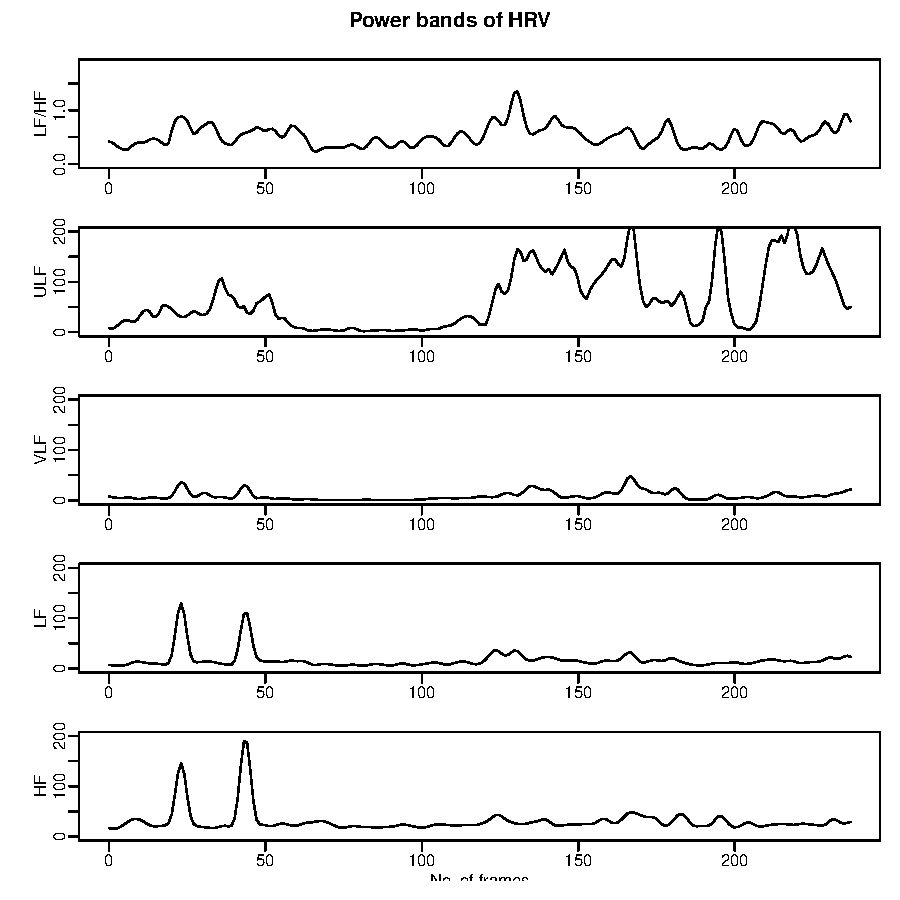
\includegraphics{figures/tutorial-plottingFreqFourier}
\caption{Plot obtained with the \textit{PlotPowerBand} for the Fourier-based 
analysis.\label{fig:examplePlotFourier}}
\end{figure}
\begin{figure}[h]
\centering
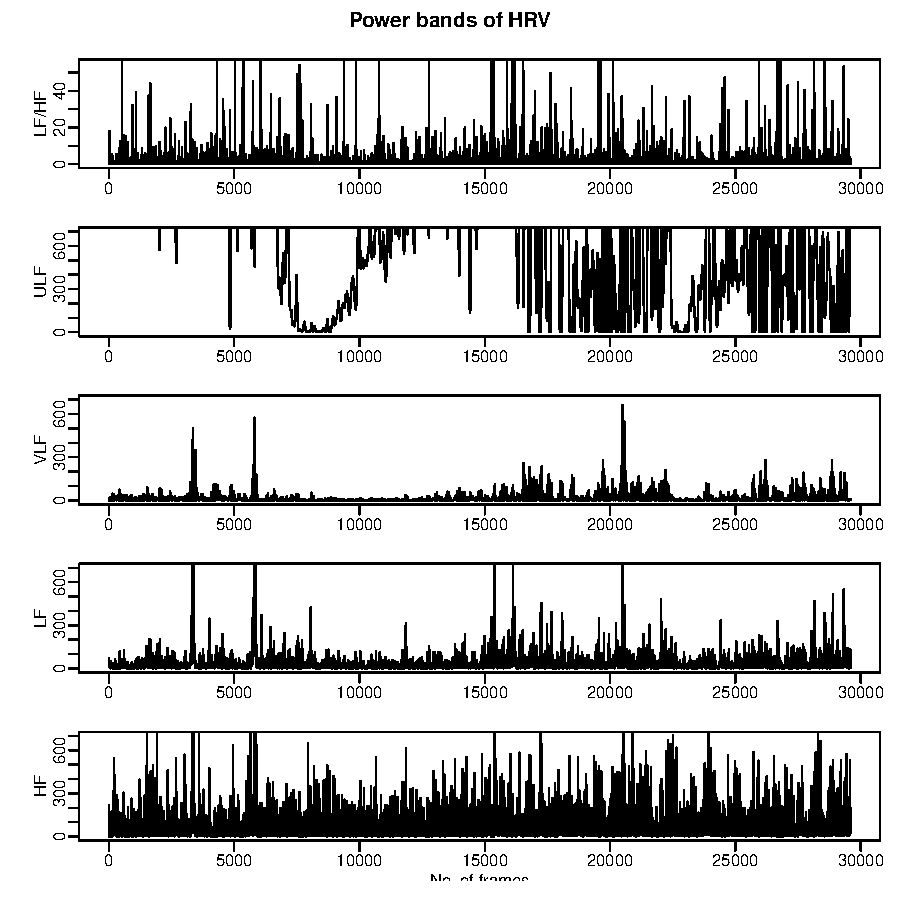
\includegraphics{figures/tutorial-plottingFreqWavelet}
\caption{Plot obtained with the \textit{PlotPowerBand} for the Wavelet-based 
analysis.\label{fig:examplePlotWave}}
\end{figure}


\subsubsection{A brief comparison: Wavelets Vs. Fourier} Figures 
\ref{fig:examplePlotFourier} and \ref{fig:examplePlotWave} illustrate some of 
the most important differences between Fourier and wavelet-based analysis. The 
most important differences may be summarized as follows:
\begin{itemize}
\item The power range is not the same when using Fourier use that when using 
wavelets due
to the windowing used in both techniques. Thus, we
should avoid direct comparisons between the numerical results obtained with 
Fourier with those obtained using wavelets.
\item The Fourier's power spectrum is smoother that the wavelet's power 
spectrum. This is a consequence of the higher temporal resolution that the 
wavelet-based analysis provides. We could try to increase Fourier's
frequency resolution by decreasing the window' size used in the analysis. The 
shorter window we use, the sharper spectrum we get. Similarly, we can 
increase/decrease temporal resolution using shorter/larger wavelets when 
performing 
wavelet-based analysis.  
\item The power spectrum obtained from the Fourier-based analysis has a smaller 
number of samples than the original signal as a consequence of the use of 
windows. Conversely, the power spectrum obtained from the wavelet-based 
analysis has the same number of samples as the original $RR$ time series.
\end{itemize}

%\subsection{Nonlinear analysis techniques\label{sec:quickNL}}

%%%%% New chapter %%%%%%
% !Rnw root = ../../tutorial.Rnw
% !Rnw root = ../../advanced.Rnw
\section{Completing our first tour}
In chapter \ref{ch:Quick} we have presented a brief description of the RHRV 
package. In this
section, we introduce some more advanced functionality of RHRV, or 
functionality that has narrower applications  than the one presented in the 
previous chapter. Thus, we will introduce some new functions 
(\textit{EditNIHR}, \textit{CalculateSpectrogram} and \textit{PlotSpectrogram}) 
and we will finish
the description of all the the function parameters introduced in the previous 
chapter. Also, further information about the 
\textit{HRVData} structure will be given.  Figure \ref{fig:completeData} shows
a detailed view of the internal organization of the HRVData structure. This 
figure
should be used as a roadmap through the explanations concerning the HRVData 
structure.

\begin{figure}[h]
\centering
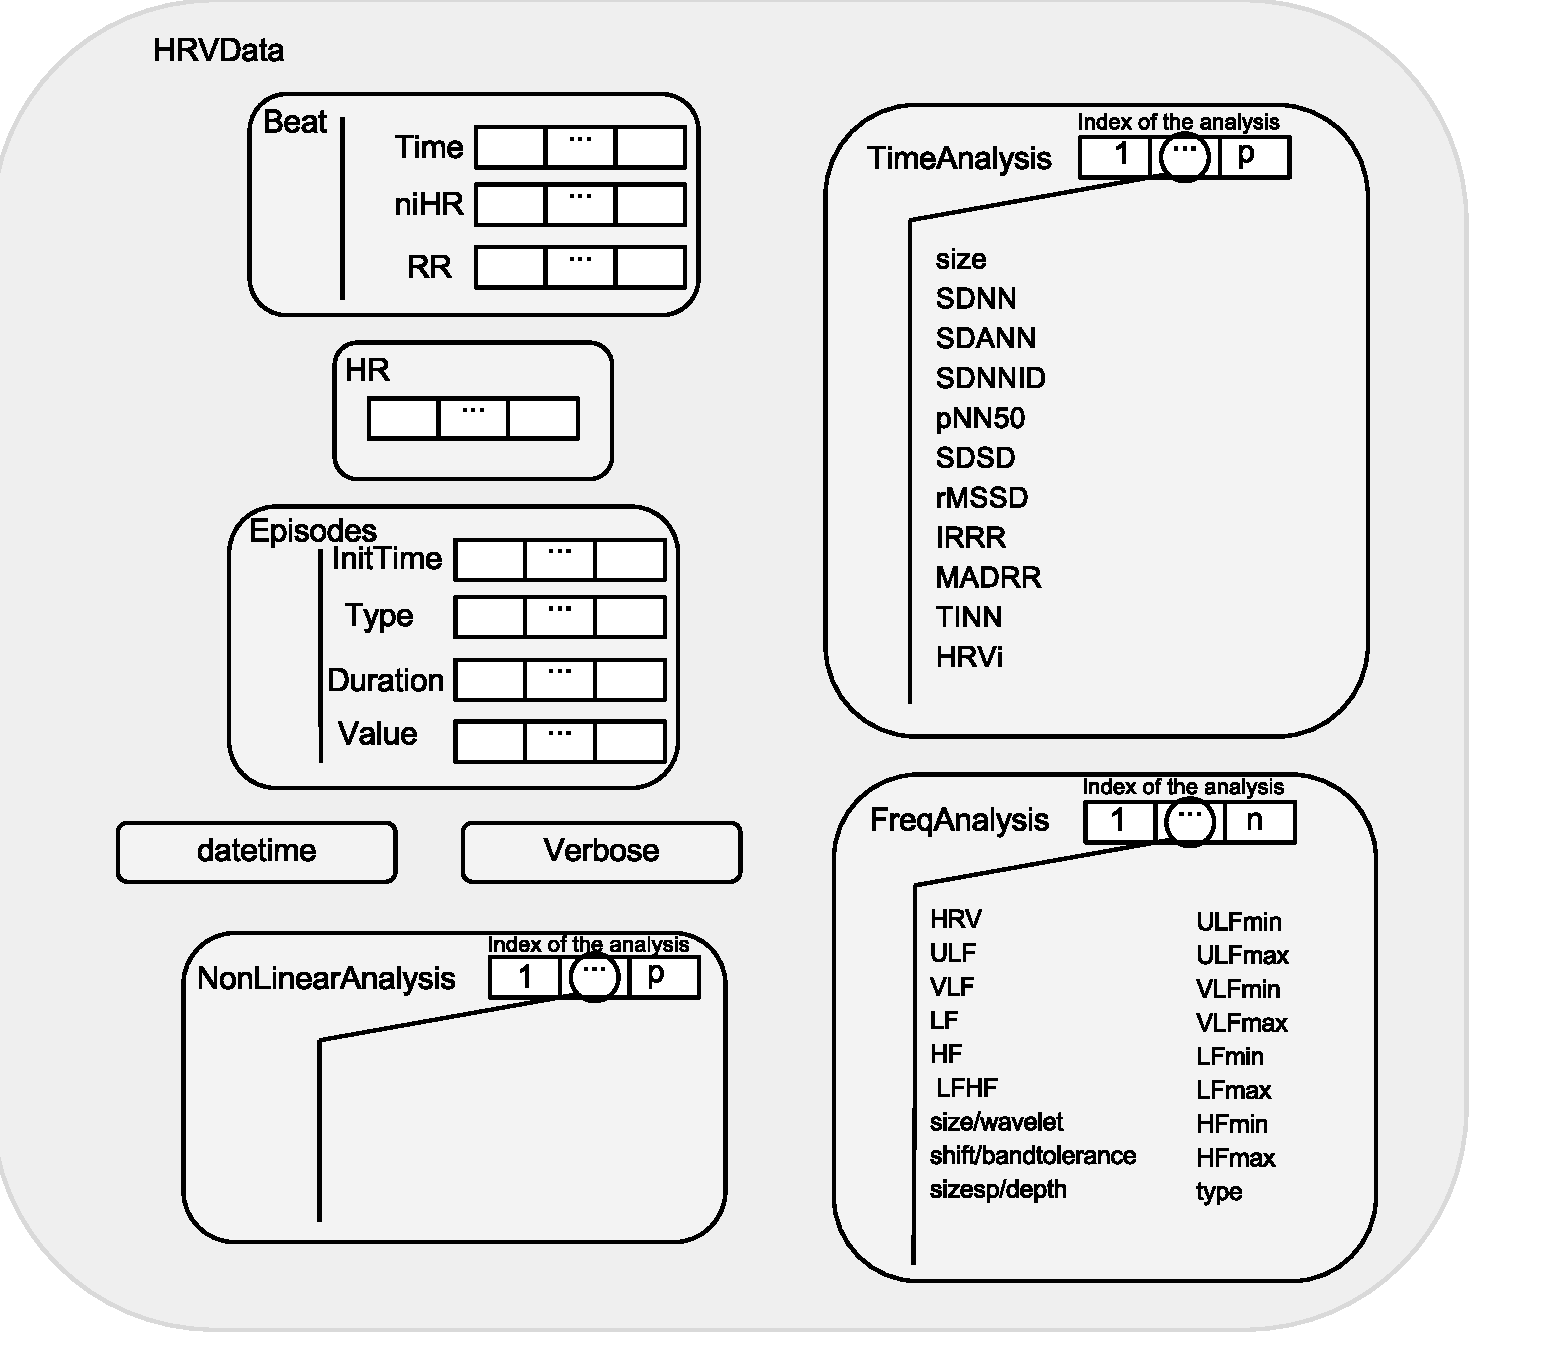
\includegraphics{figures/completeHRVData.pdf}
\caption{All the fields stored in the \textit{HRVData} 
structure.\label{fig:completeData}}
\end{figure}
\subsubsection{Creating the structure}
When a new \textit{HRVData} is created using the \textit{CreateHRVData} 
function, it contains the  following fields (among others that are not useful 
for the final user):
\begin{itemize}
\item \textit{Ext}: A string that will be used as file extension by the 
loading/writing functions included in the package. The default value is ``hrv".
\item \textit{TimeAnalysis}: This field stores the information generated using 
time-domain analysis techniques. It is is implemented as a list in the R 
language.
\item \textit{FreqAnalysis}: This field stores the  results of one or more 
frequency analysis. Frequency analysis can be based on Fourier or on wavelets. 
It is is implemented as a list in the R language.
\item \textit{NonLinearAnalysis}: This field stores the  results of one or more 
nonlinear analysis. It is is implemented as a list in the R language.
%\item \textit{Verbose}: Boolean flag that specifies if all the functions 
should return additional information (mode verbose on). The \textit{SetVerbose} 
function sets verbose mode on or off.
\end{itemize}
\subsubsection{Reading heart beats\label{sec:moreReading}} After creating the 
empty \textit{HRVData} structure  we will usually read the corresponding data 
file containing the heart beats positions. For the sake of simplicity, we keep 
on focussing on the ASCII files. The reader may have been wondering: ``what 
happens if my ASCII file is specified in milliseconds?". We shall use the  
\textit{scale} parameter to overcome this issue. By setting this parameter to 
$1$ (default value) we are indicating that the beat positions are specified in 
seconds; by setting it to $0.1$, we are indicating that the beats are in 
deciseconds and so on. The function transforms the heart beats positions to 
seconds so all the other functions can be used as before. Other interesting 
parameter that can be specified by the user is the date-time when the file was 
recorded (\textit{datetime} parameter). This is particularly useful for 
following a patient's evolution over a set of recordings. The string format for 
the \textit{datetime} parameter is ``DD/MM/YYYY HH:MM:SS". Thus, let's read the 
``example.beats" file (as in chapter \ref{ch:Quick}) specifying that  it was 
recorded on ``30/04/2012 12:00:00" in seconds:

\begin{Schunk}
\begin{Sinput}
> hrv.data = LoadBeatAscii(hrv.data, "example.beats",
+        RecordPath = "beatsFolder", scale = 1, 
+ 		   datetime = "30/04/2012 12:00:00")
\end{Sinput}
\begin{Soutput}
** Loading beats positions for record: example.beats **
   Path: beatsFolder 
   Scale: 1 
   Date: 30/04/2012
   Time: 12:00:00
   Number of beats: 17360 
\end{Soutput}
\end{Schunk}

When importing the data into the \textit{HRVData} structure, two new fields are 
created (see Figure \ref{fig:completeData}):
\begin{itemize}
\item \textit{Datetime}: Date and time associate with the record.
\item \textit{Beat}: A \textit{dataframe} object which stores the positions of 
the beats in the sub-field \textit{Time} .
\end{itemize}

\subsubsection{Constructing the time series} To compute the HRV time series the 
\textit{BuildNIHR} function is used.
 Since we have already used all the parameters of this function, we will focus 
on the \textit{HRVData structure}. As we know, this function constructs both 
the RR (Equation \ref{Eq:RR}) and instantaneous heart rate series (Equation 
\ref{Eq:RRinst}). Both series are stored in the \textit{Beat} dataframe of the 
\textit{HRVData} structure: the RR series is stored in the sub-field called 
\textit{RR} whereas the instantaneous \gls{HR} is stored in the \textit{niHR} 
sub-field (see Figure \ref{fig:completeData}).\\

\subsubsection{Filtering the time series}
The automatic removal of outliers was performed with the \textit{FilterNIHR} 
function. This function implements
an algorithm that uses adaptive thresholds for rejecting or accepting beats 
\cite{vila1997time}. The rule for beat acceptation or rejection is to compare 
the present beat with  the previous one, the following one and with an updated 
mean of the RR interval. The different adaptative thresholds establish an upper 
limit for the relative errors of each of these comparisons. The \textit{long} 
parameter allows the user to specify the number of beats that shall be used to 
calculate the updated mean (default value are 50 heartbeats). Also, the 
\textit{last} parameter permits the user to specify the initial threshold value 
in \% (default value is $13\%$). Finally, the algorithm also applies a 
comparison with acceptable physiological values. The user can specify the range 
of acceptable physiological values by using the \textit{minbpm} and 
\textit{maxbpm} (minimum beats per minute and maximum beats per minute, 
respectively). Default values are designed for human beings(\textit{minbpm}=25, 
\textit{maxbpm}=200),  but they can be specified in such a way that it may also 
be used by animal researchers. As an illustrative example we could modify the 
\textit{last} parameter in such a way that it doesn't allow quick fluctuations 
( by decreasing \textit{last} to 1\%) in our example file. Also, we could 
decrease the \textit{maxbpm} parameter to $180$ bpm. The results are shown in 
Figure \ref{fig:completeFilterNIHR} (compare it with Figure 
\ref{fig:exampleNIHR}). 

\begin{Schunk}
\begin{Sinput}
> hrv.data = FilterNIHR(hrv.data, long=50, last=1, minbpm=25, maxbpm=180)
> PlotNIHR(hrv.data)
\end{Sinput}
\end{Schunk}
\begin{figure}[h]
\centering
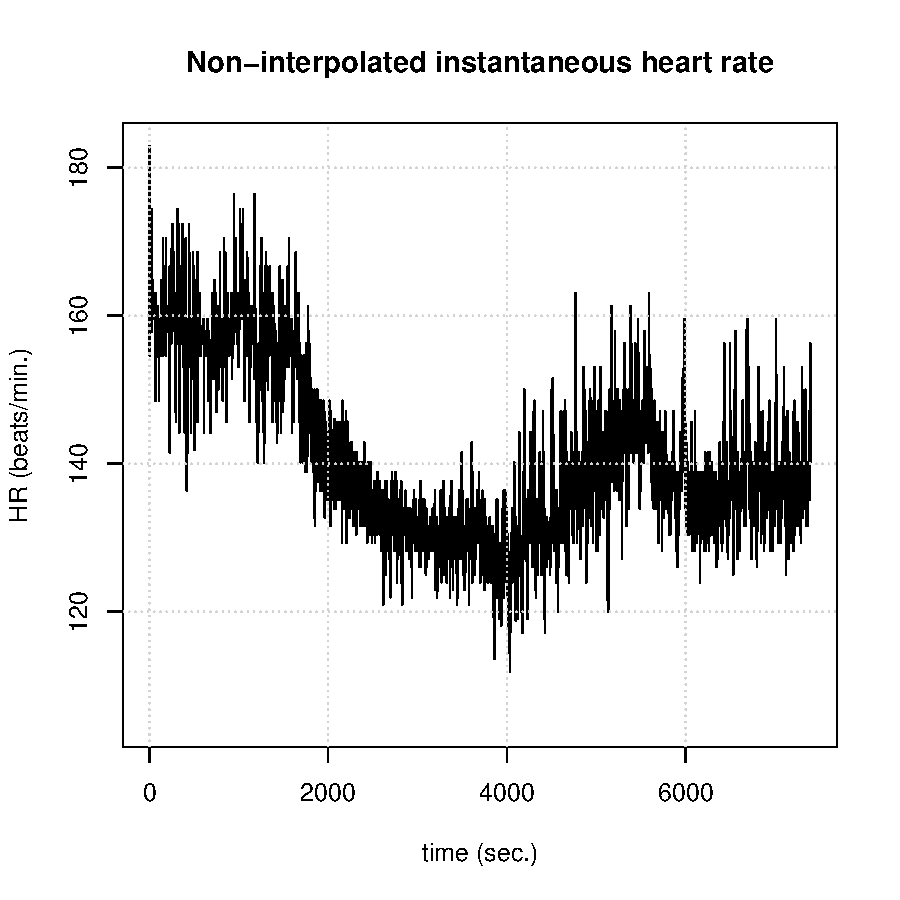
\includegraphics{figures/tutorial-completeFilterNIHR}
\caption[Modifying default values in the \textit{FilterNIHR} function]{Effects 
of the modification of the default values in the \textit{FilterNIHR} 
function.\label{fig:completeFilterNIHR}}
\end{figure}


RHRV also provides functionality for manually removing the spurious heartbeats. 
In order to delete outliers manually, a graphical editor can be used. The 
graphical editor is launched by executing the  \textit{EditNIHR} function.
\begin{Schunk}
\begin{Sinput}
> hrv.data = EditNIHR(hrv.data)
\end{Sinput}
\end{Schunk}

This interactive editor allows the user to select a rectangular area defined by 
two points that are the top left corner and bottom right corner, respectively, 
of a rectangle. (see Figure 
\ref{fig:plottingNIHR}). The points included in this rectangle can then be 
removed by pressing the ``remove outliers"  button. If we make a mistake in the 
outliers selection, we can reset the window by pressing ``clear". The 
outliers removal ends when the user presses ``End".

\begin{figure}[h]
\centering
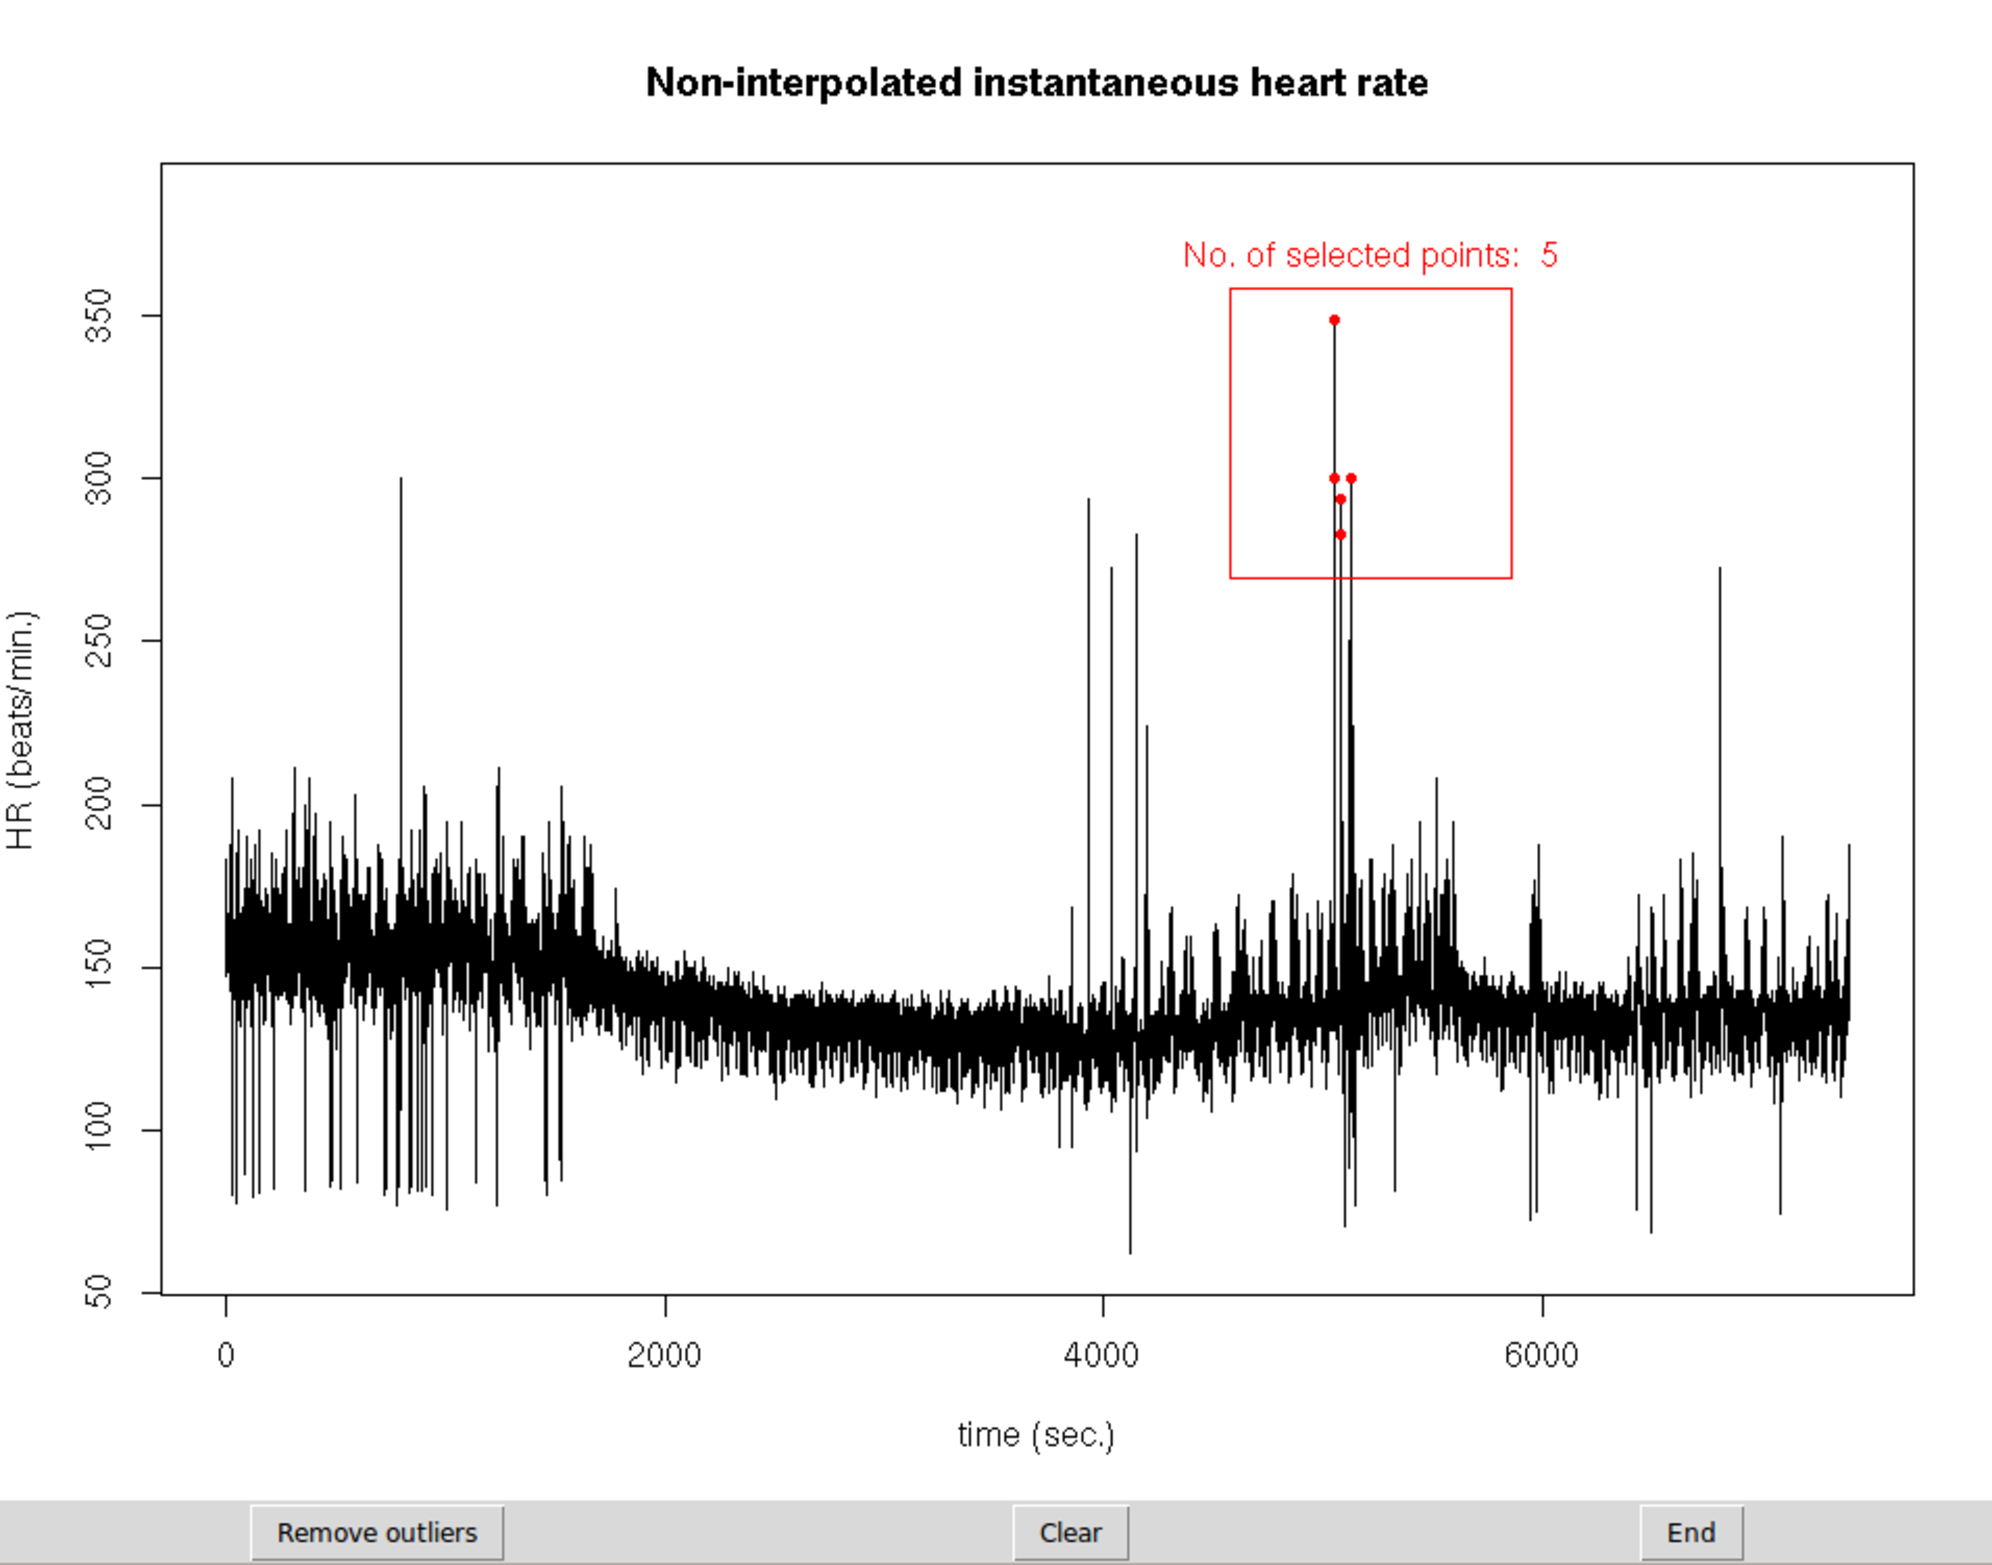
\includegraphics{figures/removing}
\caption{Manually removal of artifacts with 
\textit{EditNIHR}.\label{fig:plottingNIHR}}
\end{figure}

\subsubsection{Interpolation} The uniformly sampled \gls{HR} series is obtained 
using the \textit{InterpolateNIHR} function, which by default uses linear 
interpolation. However, it is possible to select a cubic spline interpolation 
by setting 
\textit{method = "spline"} (default value is \textit{method = "linear"}). Thus, 
as an illustrative example, let's interpolate the RR data using splines and a 
sampling frequency of $8$ Hz (This is just an illustrative example, for most of 
the situations $4$ Hz will be enough. By setting an unnecessarily high sampling 
frequency, we are overloading the computer):
\begin{Schunk}
\begin{Sinput}
> hrv.data = InterpolateNIHR (hrv.data, freqhr = 8, method = "spline")
\end{Sinput}
\end{Schunk}

This functions creates two new fields in the \textit{HRVData} structure:
\begin{itemize}
\item \textit{Freq\_HR}: Sampling frequency used in the interpolation. The 
default sampling frequency value is $4\;Hz$.
\item \textit{HR}: 	Heart Rate signal with equally spaced values at a 
certain sampling frequency obtained from the \gls{niHR} series (Figure 
\ref{fig:completeData}). 
\end{itemize}

\subsubsection{Time analysis} The \textit{CreateTimeAnalysis} function has been 
kept simple, in such a manner that the user only has to specify the window that
will be used to compute successive differences of intervals (\textit{size} 
parameter, in seconds) and the interval width of the bins that will be used to 
compute the histogram (\textit{interval} parameter, in milliseconds), as shown 
in chapter \ref{ch:Quick}. \\

This functions fills (one position of) the \textit{TimeAnalysis} in the 
\textit{HRVData} structure by computing the following parameters: SDNN, SDANN, 
SDNNIDX, pNN50, rMSSD, IRRR, MADRR, TINN and HRVi (see Figure 
\ref{fig:completeData} and section \ref{sec:timedomain}). The size of the 
window involved in the computations is also stored in the \textit{size} field.


\subsubsection{Frequency analysis} All the main \textit{parameters} of the 
\textit{CalculatePowerBand} function have already been used in chapter 
\ref{ch:RHRV}. As shown in Figure \ref{fig:completeData}, the 
\textit{CalculatePowerBand} function fills the corresponding  
\textit{FreqAnalysis} data structure with the following fields:
\begin{itemize}
\item \textit{Type}: a string identifying the type of analysis that has been 
used. The possible values are either \textit{``fourier"} or \textit{``wavelet"}.
\item \textit{ULFmin}, \textit{ULFmax}, \textit{VLFmin}, \textit{VLFmax}, 
\textit{LFmin}, \textit{LFmax}, \textit{HFmin} and \textit{HFmax}: These fields 
store the boundaries of each frequency band.
\item \textit{ULF}, \textit{VLF}, \textit{LF} and \textit{HF}:   These fields 
store the spectrogram of the HR signal in the  ULF, VLF, LF and HF bands, 
respectively.
\item \textit{HRV}: Stores the total energy of the signal as a function of 
time. This Energy time series is estimated from the spectrogram signal.
\item \textit{LFHF}: Stores the LF/HF ratio (Section \ref{sec:analysisTechn}) 
by dividing the LF time series by the HF time series.
\end{itemize}
Some additional parameters are incorporated to the \textit{FreqAnalysis} 
structure depending on the type of analysis used. When using the \gls{STFT}, 
the \textit{size}, \textit{shift} and \textit{sizesp} fields store information 
about the window, the window shift, and the number of points per \gls{DFT} that 
have been used. When using the Wavelet transform, the \textit{wavelet}, 
\textit{ bandtolerance} and \textit{depth} fields store information about the 
mother Wavelet and the tolerance used, as well as the number of levels that the 
algorithm has descended in the \gls{MODWPT} tree \cite{waveletBiosignals}, 
\cite{waveletArticle}.\\

RHRV provides another function for computing the spectrogram without being 
restricted to the four bands: \gls{ULF}, \gls{VLF}, \gls{LF} and \gls{HF}. This 
function, called \textit{CalculateSpectrogram}, uses the \gls{STFT} approach. 
Thus, the user has to specify the size of window (\textit{size} parameter), the 
displacement of window  (\textit{shift}) and the zero-padding 
(\textit{sizesp}), as in the \textit{CalculatePowerBand} function. The 
spectrogram is returned in a real matrix in a way that, as the number of the 
row increases, the time increases and, as the column's number increases, the 
frequency increases. This matrix
is not stored in the \textit{HRVData} structure since it can be very expensive 
in terms of 
memory. As an example, let's compute the spectrogram of the example file with 
the same parameters used with the \textit{CalculatePowerBand} function:
\begin{Schunk}
\begin{Sinput}
> # Plotting Fourier analysis
> spectrogram = CalculateSpectrogram( hrv.data ,size = 300,
+  shift = 30, sizesp = 2048)
\end{Sinput}
\end{Schunk}
The user can obtain a graphical representation of the spectrogram by using the 
\textit{image} R function. Alternatively, the user can use the 
\textit{PlotSpectrogram} function, that also returns the spectrogram matrix 
(see Figure \ref{fig:plottingSpectrogram}). By using the \textit{scale} 
function, the
user may choose a linear axis (``linear") or a logarithmic axis 
(``logarithmic"). The user must also specify the 
\textit{size}, \textit{shift} and \textit{sizesp} parameter. 
\begin{Schunk}
\begin{Sinput}
> # Plotting wavelet analysis
> spectrogram = PlotSpectrogram(HRVData=hrv.data, size=300, shift=60,
+  sizesp=2048)
\end{Sinput}
\end{Schunk}
Note that most part of the energy of the figure \ref {fig:plottingSpectrogram} 
is concentrated in the low frequencies. To obtain a more
detailed graphic in this zone of the spectrum, we can use the 
\textit{freqRange} parameter. For example, if we wish to plot the spectrum in 
the $[0,0.2]\;Hz$ band, we write:
\begin{Schunk}
\begin{Sinput}
> # Plotting wavelet analysis
> PlotSpectrogram(HRVData=hrv.data, size=300, shift=60, 
+ 	sizesp=2048,freqRange = c(0,0.2))
\end{Sinput}
\end{Schunk}
The result of this script is shown in figure \ref{fig:plottingSpectrogram2}.
\begin{figure}[h]
\centering
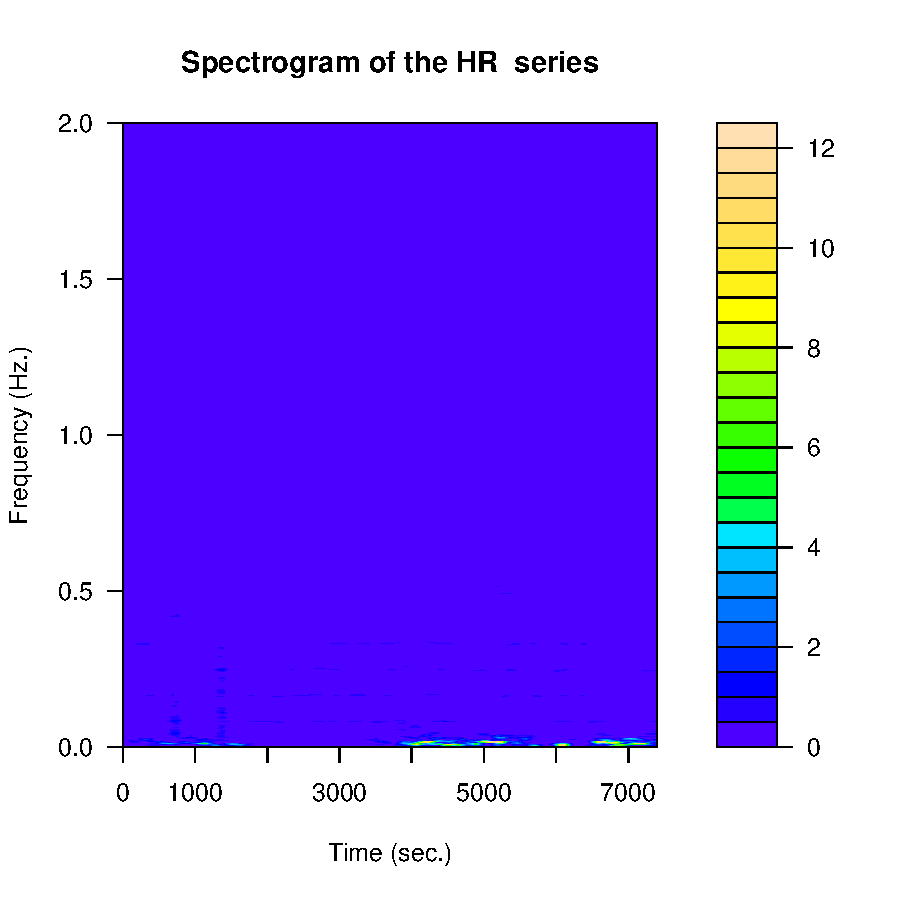
\includegraphics{figures/tutorial-plottingSpectrogram}
\caption{Plot obtained with the \textit{PlotSpectrogram} 
function.\label{fig:plottingSpectrogram}}
\end{figure}


\begin{figure}[h]
\centering
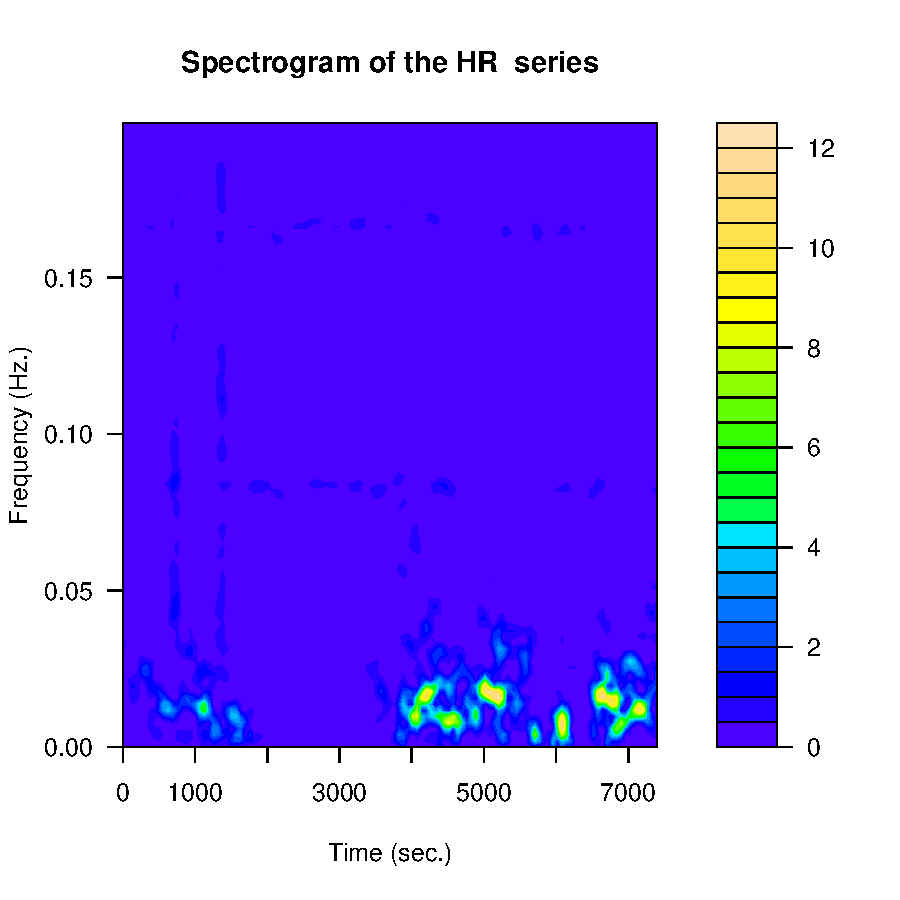
\includegraphics{figures/tutorial-plottingSpectrogram2}
\caption[Plotting with the \textit{PlotSpectrogram} function using the 
\textit{freqRange} parameter]{Plot obtained with the \textit{PlotSpectrogram} 
function and the \textit{freqRange} parameter.\label{fig:plottingSpectrogram2}}
\end{figure}

%\subsubsection{Nonlinear analysis} 

% !Rnw root = ../../advanced.Rnw
\chapter{Advanced use of  RHRV\label{ch:RHRV}}

\section{Reading several file formats\label{sec:fileFormats}}
% !Rnw root = advanced.Rnw
 RHRV provides a lot of functionality for importing data files containing heart 
beats positions. Supported formats include ASCII (\textit{LoadBeatAscii} 
function), EDF (\textit{LoadBeatEDFPlus}), Polar (\textit{LoadBeatPolar}), 
Suunto (\textit{LoadBeatSuunto}) and WFDB data files (\textit{LoadBeatWFDB}) 
\cite{mitbih}. We have already dealt with the \textit{LoadBeatASCII} function. 
In this section, we will discuss the remaining functions for reading heart beat 
data.

\subsection{Reading \textit{RR} files} There exist another \textit{RHRV} 
function that reads ASCII files:  the \textit{LoadBeatRR} function. This 
function reads ASCII files storing the \textit{RR} intervals (and not the heart 
beat times). The parameters of the \textit{LoadBeatRR} function are exactly the 
same as those of the \textit{LoadBeatAscii} function, that is:
\begin{Schunk}
\begin{Sinput}
> LoadBeatRR(HRVData, RecordName, RecordPath=".", scale = 1, 
+       datetime = "1/1/1900 0:0:0")
\end{Sinput}
\end{Schunk}
\subsection{Reading files in WFDB format} PhysioNet \cite{physioNet} is a free 
web resource that provides large collections of recorded physiologic signals 
(PhysioBank) and related open-source software (PhysioToolkit). In most cases, a 
record from PhysioBank consists of at least three files, which are named using 
the record name followed by different extensions that indicate their content. 
Almost all records include a binary .dat  file, containing digitized samples of 
one or more signals. The .hea (header) file is a short text file that describes 
the signals. Most records include one or more binary annotation files. For 
example, .qrs files contain an annotation for each QRS complex (heart beat) in 
the recording; .apn files contain apnea annotations; etc. For the sake of 
simplicity, we call ``WFDB file" (WaveForm DataBase) to such a collection of 
files containing data on the same recording \cite{mitbih}. Further details 
about PhysioBank can be found in the Physionet website. \\

The RHRV package provides the \textit{LoadBeatWFDB} function for reading WFDB 
files. This function takes as input parameters the name of the WFDB file to be 
used without any extension (\textit{RecordName} argument), the  relative path 
of the file (\textit{RecordPath} argument) and the extension of the file with 
the heart beats annotations (\textit{annotator}, its default value is ``qrs", 
so in most cases the user won't have to specify it). As an example, we are 
going to
 create a data structure that will read the ``a03" register from the 
PhysioBank's Apnea-ECG database \cite{penzel2000apnea}.
\begin{Schunk}
\begin{Sinput}
> hrv.wfdb = CreateHRVData()
> hrv.wfdb = SetVerbose(hrv.wfdb, TRUE)
> hrv.wfdb = LoadBeatWFDB(hrv.wfdb, "a03", RecordPath =".",
+  annotator = "qrs")
\end{Sinput}
\begin{Soutput}
** Loading beats positions for record: a03 **
   Path: . 
   Opening header file: a03.hea 
      No time information in header: 00:00:00 
      No date information in header: 01/01/1900 
   Date: 01/01/1900
   Time: 00:00:00
   Number of beats: 34254 
\end{Soutput}
\end{Schunk}

\subsection{Other formats} Since the remaining functions have a similar 
behaviour than those we have already discussed, we will just discuss their 
prototypes. The \textit{LoadBeatEDFPlus} function allows the user to read EDF+ 
(European Data Format) data \cite{kemp2003european}. Its format is similar to 
the \textit{LoadBeatWFDB} function:
\begin{Schunk}
\begin{Sinput}
> LoadBeatEDFPlus(HRVData, RecordName, RecordPath = ".", 
+ 	annotationType ="QRS")
\end{Sinput}
\end{Schunk}
Finally, RHRV provides functionality for reading Polar and Suunto files with 
the \textit{LoadBeatPolar} and \textit{LoadBeatSuunto} functions. These 
functions only receive as arguments the record name and the record path:
\begin{Schunk}
\begin{Sinput}
> LoadBeatPolar(HRVData, RecordName, RecordPath=".")
> LoadBeatSuunto(HRVData, RecordName, RecordPath=".")
\end{Sinput}
\end{Schunk}

\subsection{A general function} The \textit{LoadBeat} function provides a 
common interface to access all the functions responsible for loading heart 
beats. Thus, the prototype of the \textit{LoadBeat} function contains all the 
\textit{parameters} needed for the loading functions. It also offers the 
\textit{fileType} parameter so the user can specify which kind of file is going 
to be readed. Depending on the \textit{fileType} value, the \textit{LoadBeat} 
function delegates on one of the previous loading functions. The possible 
values of the \textit{fileType} parameter and the function that is called are 
summarized in table \ref{tab:loadbeat}.

\begin{table}
\begin{center}
\begin{tabular}{ |c| c| }
\hline
\textbf{fileType}&\textbf{function called}\\
\hline
``WFDB"&\textit{LoadBeatWFDB}\\
``Ascii"&\textit{LoadBeatAscii}\\
``RR"&\textit{LoadBeatRR}\\
``Polar"&\textit{LoadBeatPolar}\\
``Suunto"&\textit{LoadBeatSuunto}\\
``EDFPlus"&\textit{LoadBeatEDFPlus}\\
\hline
\end{tabular}
\caption{\textit{LoadBeat} operation depending on the \textit{fileType} 
parameter.}
\label{tab:loadbeat}
\end{center}
\end{table}
Thus, if we want to read a WFDB file, we could use either the  
\textit{LoadBeatWFDB} function or the \textit{LoadBeat} function:
\begin{Schunk}
\begin{Sinput}
> hrv.wfdb = CreateHRVData()
> hrv.wfdb = SetVerbose(hrv.wfdb, TRUE)
> hrv.wfdb = LoadBeat(hrv.wfdb, fileType = "WFDB", "a03", RecordPath =".", 
+ annotator = "qrs")
\end{Sinput}
\begin{Soutput}
** Loading beats positions for record: a03 **
   Path: . 
   Opening header file: a03.hea 
      No time information in header: 00:00:00 
      No date information in header: 01/01/1900 
   Date: 01/01/1900
   Time: 00:00:00
   Number of beats: 34254 
\end{Soutput}
\end{Schunk}

\section{Performing analysis in different intervals of a recording\label{sec:episodeInformations}}
% Rnw root = advanced.Rnw
Intervals of the \gls{HR} time series with pathophysiological interest may be 
annotated in the so-called episode files. For example, it may be interesting to 
compare the heart rate series before, during and after an apnea episode (apneas 
are cessations of a patient's respiratory airflow during the nocturnal rest) 
\cite{lado2012nocturnal}. Such a study could be useful for searching for 
significant differences
in the HRV caused by the apneas. The RHRV package provides functions for 
loading episode information. The supported formats for this information are 
either ASCII (\textit{LoadEpisodesAscii}) or
WFDB (\textit{LoadApneaWFDB}). Episodes may also be added programmatically to 
the time series using the \textit{AddEpisodes} function. All episodes are 
stored under the \textit{Episodes} field of the \textit{HRVData} structure (see 
Figure \ref{fig:completeData}). The plotting functions allow the user to 
include episodic information in the graphics. We will discuss all this points 
in more detail below.\\
\subsection{AddEpisodes\label{par:AddEpisodes}} The simplest way of adding 
episodic information is using the \textit{AddEpisodes} function. 
\textit{AddEpisodes} adds information of episodes by specifying the initial 
times of each episode (\textit{InitTimes} argument, in seconds), the names of 
the episodes (\textit{Tags}), the duration of each episode (\textit{Durations}, 
in seconds) and a numerical identifier for each episode(\textit{Values}). The 
\textit{Values} field is useful for those episodes
that store some numerical values. For example, an apnea episode could store 
information
about the Oxygen saturation level in the \textit{Values} field. Note that all 
the parameters specified by the user will be stored in the \textit{HRVData} 
structure in its corresponding fields as shown in Figure 
\ref{fig:completeData}.\\

Let us read our example file ``example.beats" and add three episodes to it: a 
first type ``A" episode in the $[700,1600]\;s$ interval; a second episode of 
the same type as the first one (``A") in the $[5000,5600]\;s$ interval; and a 
third episode in the $[2000,4500]\;s$ interval of type ``B":

\begin{Schunk}
\begin{Sinput}
> hrv.data = CreateHRVData( )
> hrv.data = LoadBeatAscii(hrv.data,"example.beats","beatsFolder")
> hrv.data = SetVerbose(hrv.data,TRUE)
> hrv.data = AddEpisodes(hrv.data, InitTimes = c(700,5000,2000),
+ Tags = c("A","A","B"), Durations = c(900,600,2500), Values = c(0,0,0))
\end{Sinput}
\begin{Soutput}
** Adding new episodes **
   Added 3 episodes from file
   Number of episodes: 3 
\end{Soutput}
\end{Schunk}


\subsection{Plotting episodic information} The \textit{plotHR} and  
\textit{PlotNIHR} functions allow the user to include episodic information in 
the plot. The user can specify a list of tags to specify which episodes are 
included in the plot (\textit{Tag} parameter). \textit{Tag=``all"} plots all 
episodes present in the data. Thus we could execute, after the code of the 
previous paragraph:
\begin{Schunk}
\begin{Sinput}
> hrv.data = BuildNIHR(hrv.data)
> # plot all tags
> PlotNIHR(hrv.data, Tag="all")
\end{Sinput}
\end{Schunk}
\begin{Schunk}
\begin{Sinput}
> hrv.data  = InterpolateNIHR(hrv.data, freqhr = 4)
> # Plot only the "A" episodic information 
> PlotHR(hrv.data , Tag=c("A"))
\end{Sinput}
\end{Schunk}

The plots obtained with \textit{PlotNIHR} and \textit{PlotHR} are shown in 
Figures \ref{fig:plottingEpisodicNIHR} and \ref{fig:plottingEpisodicHR}, 
respectively.
\begin{figure}[h]
\centering
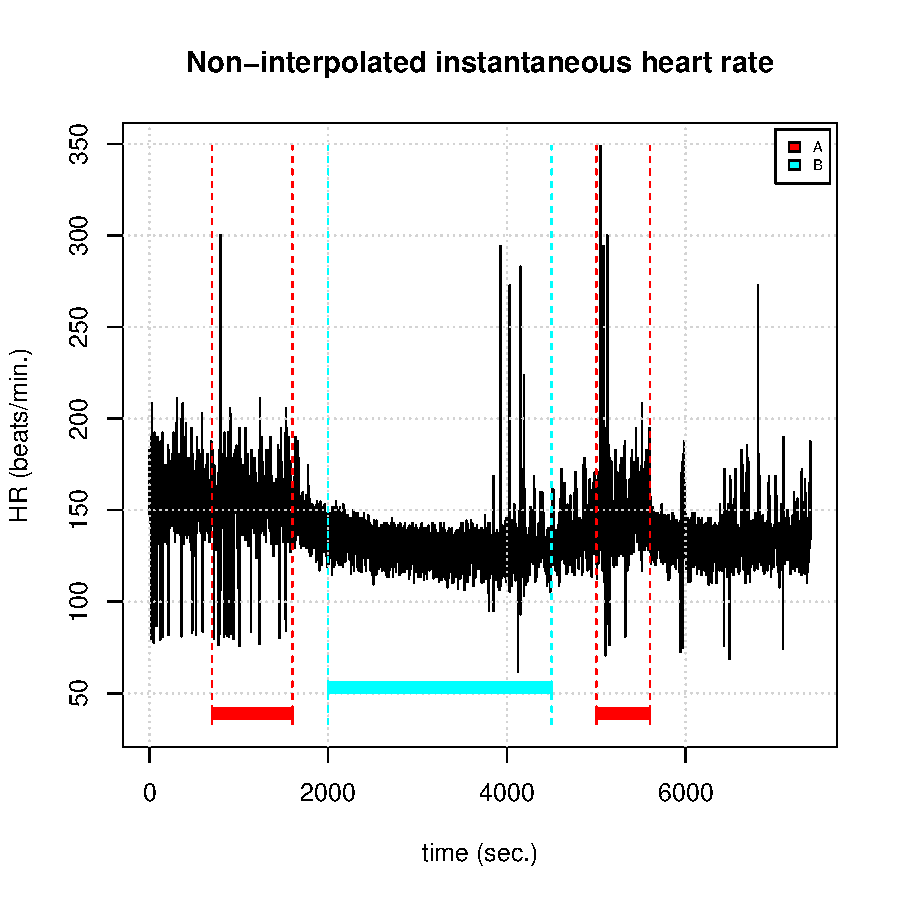
\includegraphics{figures/tutorial-plottingEpisodicNIHR}
\caption{Episodic information in the Non interpolated Heart Rate time 
series.\label{fig:plottingEpisodicNIHR}}
\end{figure}
\begin{figure}[h]
\centering
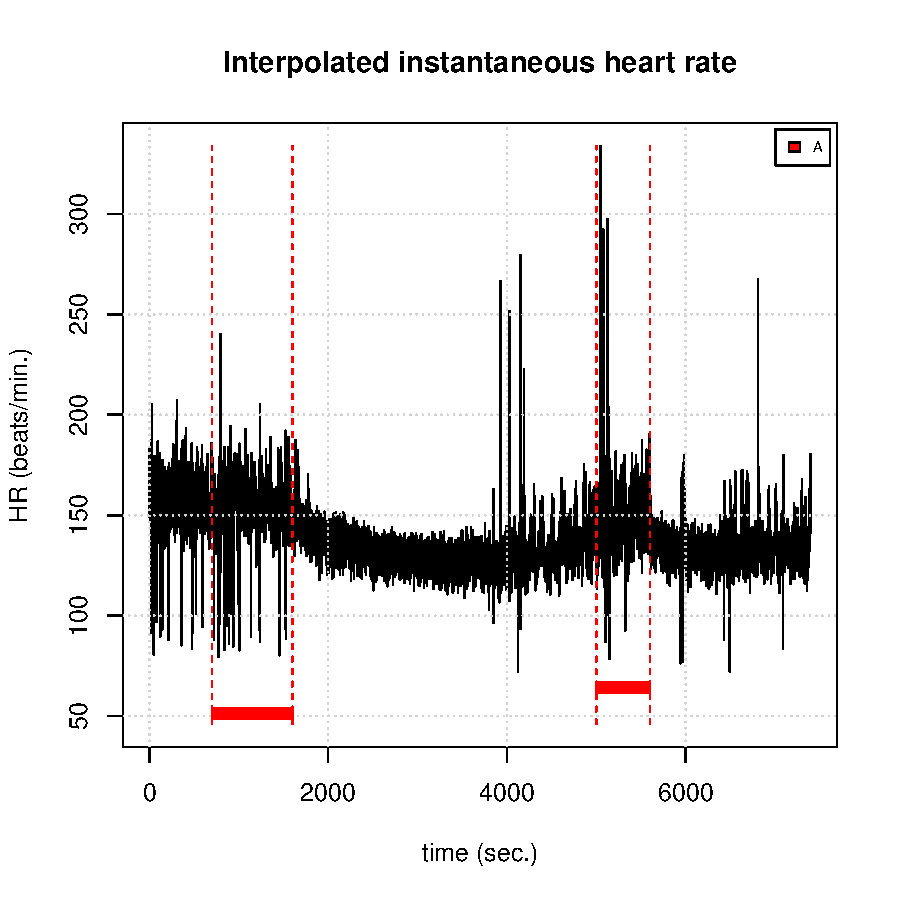
\includegraphics{figures/tutorial-plottingEpisodicHR}
\caption{Episodic information in the interpolated Heart Rate time 
series.\label{fig:plottingEpisodicHR}}
\end{figure}


RHRV is also capable of  including episodic information when representing the 
spectrograms obtained with the
\textit{CalculatePowerBand}. For this purpose, the {PlotPowerBand} includes the 
\textit{Tag} input parameter. Thus, if we want to perform a frequency analysis 
and plot the power bands with the episodic information that we have added in 
the previous paragraphs, we could execute:
\begin{Schunk}
\begin{Sinput}
> hrv.data = CreateFreqAnalysis(hrv.data)
> # perform frequency analysis
> hrv.data = CalculatePowerBand( hrv.data , indexFreqAnalysis= 1,
+  type = "wavelet", wavelet = "la8", bandtolerance = 0.01, relative = FALSE)
> # plot episodic information
> PlotPowerBand(hrv.data, indexFreqAnalysis = 1, ymax = 5000, ymaxratio = 50, 
+   			Tag = "all")
\end{Sinput}
\end{Schunk}
The resulting plot is shown in Figure \ref{fig:episodicFrequency}.
\begin{figure}[h]
\centering
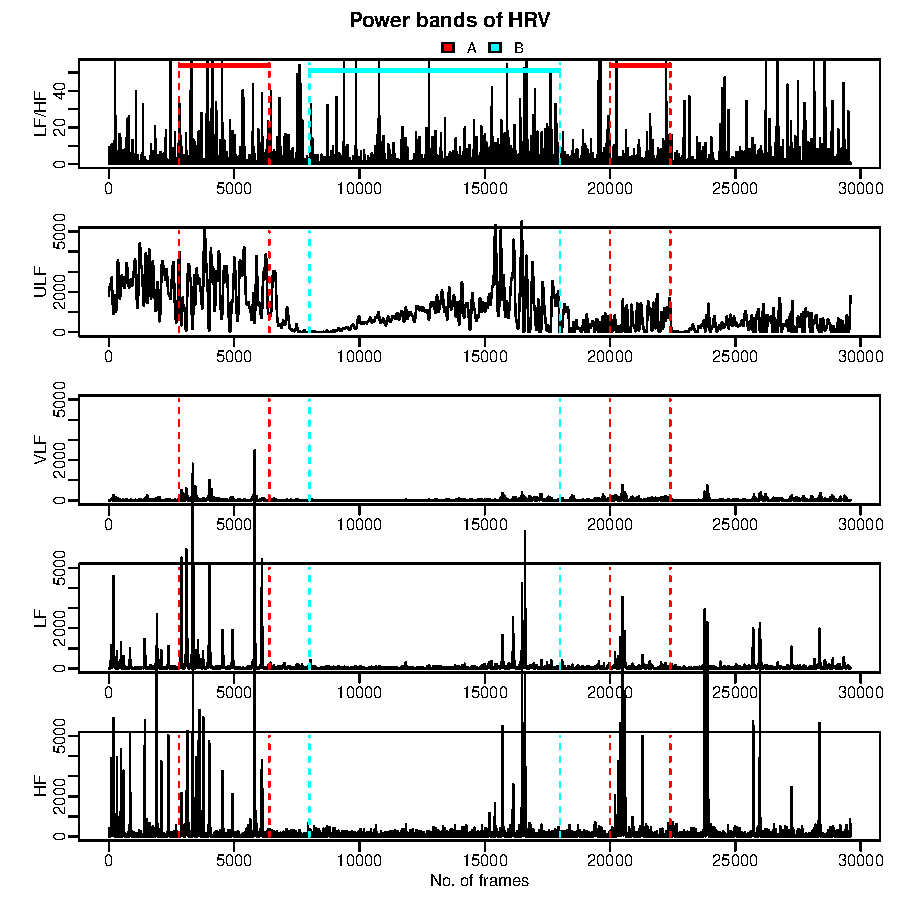
\includegraphics{figures/tutorial-episodicFrequency}
\caption{Episodic information in all the power 
bands.\label{fig:episodicFrequency}}
\end{figure}

\subsection{LoadEpisodesAscii} The \textit{LoadEpisodesAscii} allows the user 
to read episodic information stored in an ASCII file saving it into the 
\textit{HRVData} data structure. The expected format of each line is:\\
\begin{center}
\begin{tabular}{ c c c c }
InitTime &Tag & Duration&  Value\\
\hline
HH:MM:SS  &``Tag name"& double &integer
\end{tabular}
\end{center} 
The first column is the start time of the episode with the ``HH:MM:SS" format. 
The second column serves the same purpose as the \textit{Tag} parameter in 
\textit{AddEpisodes}. The third column specifies the duration of the episode in 
seconds. Finally, the forth column assigns a  numerical value for each episode 
( the same function performed by the \textit{Value} parameter in the 
\textit{AddEpisodes} function). \\

It must be taken into account that the \textit{LoadEpisodesAscii} skips the 
first line of the ASCII file because it assumes that the first line will 
contain a header ( the format of this header does not really matter). If there 
is no header line in the file, the user
can specify it to the function using the \textit{header} parameter (by default, 
it is
setted to TRUE).\\

As an example, we are going to create an ASCII file containing the same 
information as the episodes ``A" and ``B" that we programmatically introduced 
in the \textit{AddEpisodes}(\ref{par:AddEpisodes}) paragraph. We will also add 
information about a "C" episode that the \textit{LoadEpisodesAscii} will skip. 
We shall call this file ``annotationsFile.txt". This file will have the 
following content:
\begin{center}
\begin{tabular}{ c c c c }
InitTime&  Type & Duration&  Value\\
00:11:40 & "A"& 900 &1\\
01:23:20 & ``A" &600 &2\\
00:33:20 & "B" &2500 &3\\
01:00:00 & "C"& 100 &4\\
\end{tabular}
\end{center} 

The \textit{LoadEpisodesAscii} function takes as input parameters: the absolute 
path to the episodes file to be readed (\textit{FileName}), the types of 
episodes that should be readed (\textit{Tag}) and the time (``HH:MM:SS") at 
which the recording began (\textit{InitTime}). This last parameter enables 
reading those files in which the initial time of episodes was specified in 
absolute time, and not relative to the start of the recording. Since we wrote 
relative times in the ASCII file, we should use \textit{InitTime=``0:0:0"}. 
Thus, in order to read just the episodes tagged as ``A" from our file, we could 
write:

%\textbf{TODO: falla al leer dos tags!!}

\begin{Schunk}
\begin{Sinput}
> hrv.data = CreateHRVData( )
> hrv.data = LoadBeatAscii(hrv.data,"example.beats","beatsFolder")
> hrv.data = SetVerbose(hrv.data,TRUE)
> hrv.data = LoadEpisodesAscii(hrv.data,Tag=c("A"),InitTime="0:0:0",
+ FileName="beatsFolder/annotationsFile.txt")
\end{Sinput}
\begin{Soutput}
** Loading episodes file: beatsFolder/annotationsFile.txt **
   Path: . 
   Tag: A 
   Initial time: 00:00:0.000
   Data includes values associated to episodes
   Loaded 2 episodes from file
   Number of episodes: 2 
\end{Soutput}
\end{Schunk}
\subsection{LoadApneaWFDB} The \textit{LoadApneaWFDB} function allows the user 
to load apnea annotations from a WFDB file (the user must ensure that there is 
a file with the .apn extension between the WFDB recording's files). The 
function takes as input parameters the name of the WFDB file 
(\textit{RecordName}), the path to the WFDB file (\textit{RecordPath}) and a 
name for the apnea episodes (\textit{Tag}, its default value is ``APNEA"). The 
use of this function requires the installation of the WFDB tools (see chapter 
\ref{ch:installation}).

As an illustrative example, we are going to read the apnea episodes for the 
``a03" file of the ApneaECG database from PhysioBank (see the \textit{Reading 
files in WFDB format} paragraph). The plot of the non interpolated \gls{HR} 
series is shown in figure \ref{fig:loadingApneaEpisodes}.
\begin{Schunk}
\begin{Sinput}
> hrv.wfdb = CreateHRVData()
> hrv.wfdb = SetVerbose(hrv.wfdb, TRUE)
> hrv.wfdb = LoadBeat(hrv.wfdb, fileType = "WFDB", "a03", RecordPath =".", 
+                     annotator = "qrs")
\end{Sinput}
\begin{Soutput}
** Loading beats positions for record: a03 **
   Path: . 
   Opening header file: a03.hea 
      No time information in header: 00:00:00 
      No date information in header: 01/01/1900 
   Date: 01/01/1900
   Time: 00:00:00
   Number of beats: 34254 
\end{Soutput}
\begin{Sinput}
> hrv.wfdb = LoadApneaWFDB(hrv.wfdb, RecordName="a03",Tag="Apnea",
+ RecordPath=".")
\end{Sinput}
\begin{Soutput}
** Loading apnea episodes for record: a03 **
   Path: . 
   Header info already present for: a03 
   Command: rdann -r a03 -a apn 
   Number of labels: 518 
** Adding new episodes **
   Added 11 episodes from file
   Number of episodes: 11 
\end{Soutput}
\begin{Sinput}
> hrv.wfdb = BuildNIHR(hrv.wfdb)
\end{Sinput}
\begin{Soutput}
** Calculating non-interpolated heart rate **
   Number of beats: 34254 
\end{Soutput}
\begin{Sinput}
> PlotNIHR(hrv.wfdb,Tag="all")
\end{Sinput}
\begin{Soutput}
** Plotting non-interpolated instantaneous heart rate **
   Number of points: 34254 
   Episodes in plot: Apnea 
   No of episodes: 11 
   No of classes of episodes: 1 
\end{Soutput}
\end{Schunk}

\begin{figure}[h]
\centering
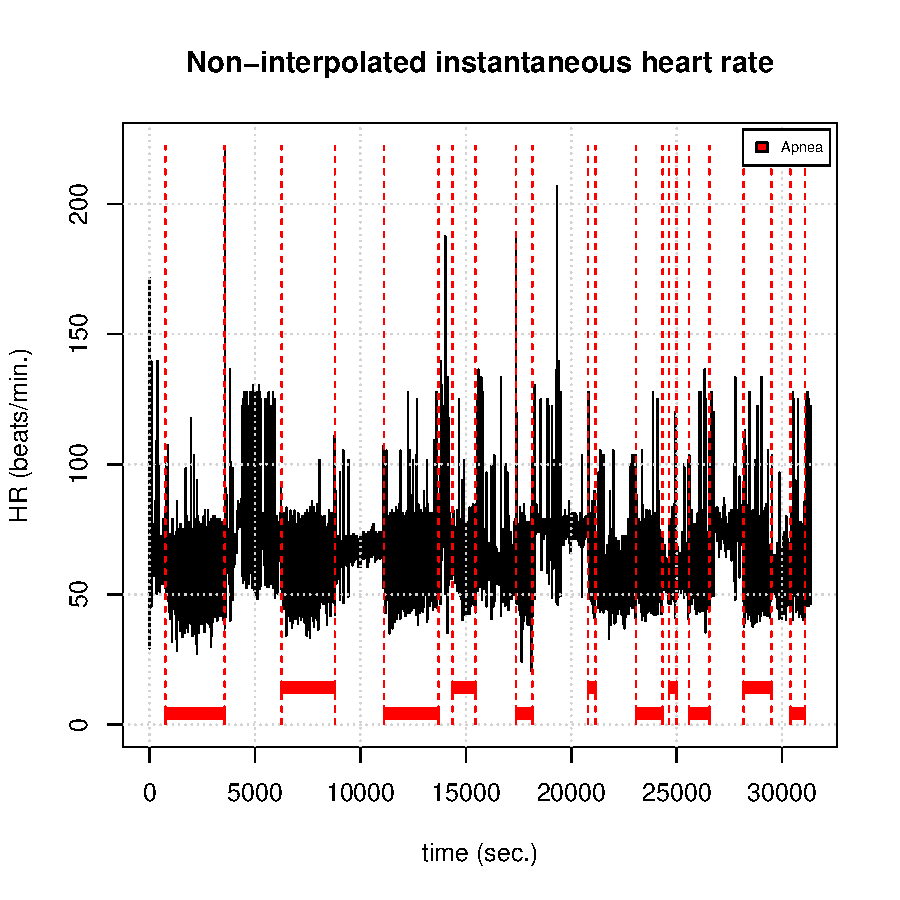
\includegraphics{figures/tutorial-loadingApneaEpisodes}
\caption{Loading Apnea episodes using the \textit{LoadApneaWFDB} 
function.\label{fig:loadingApneaEpisodes}}
\end{figure}

\subsection{Analyzing HRV inside and outside the episodes}
 RHRV provides basic functionality for comparing data inside and outside each
episode. The simplest function that the user can use for this purpose is the 
\textit{SplitHRbyEpisodes} function, that splits the  interpolated heart rate 
series into two vectors containing samples inside (the ``InEpisodes" vector) 
and outside the episode (the ``OutEpisodes" vector) specified in
the \textit{Tag} argument. For example, if we want to compare the \gls{HR} 
series inside and outside the apnea episodes from the ``a03" file, we could use:
\begin{Schunk}
\begin{Sinput}
> # remember to interpolate the Heart Rate series!!
> hrv.wfdb = InterpolateNIHR (hrv.wfdb, freqhr = 4)
\end{Sinput}
\begin{Soutput}
** Interpolating instantaneous heart rate **
   Frequency: 4Hz
   Number of beats: 34254 
   Number of points: 125383 
\end{Soutput}
\begin{Sinput}
> splitting.data = SplitHRbyEpisodes(hrv.wfdb, Tag = c("Apnea"))
\end{Sinput}
\begin{Soutput}
** Splitting heart rate signal using episodes **
   Using episodes with tag: Apnea 
   Number of episodes: 11 
   Inside episodes: 58919 points
   Outside episodes: 66464 points
\end{Soutput}
\end{Schunk}
It's straightforward to use a statistical function for comparing both vectors. 
For example:
\begin{Schunk}
\begin{Sinput}
> cat("comparing the mean inside and outside Apnea episodes...\n")
\end{Sinput}
\begin{Soutput}
comparing the mean inside and outside Apnea episodes...
\end{Soutput}
\begin{Sinput}
> cat("Apnea mean: ",mean(splitting.data$InEpisodes),"\n")
\end{Sinput}
\begin{Soutput}
Apnea mean:  61.94101 
\end{Soutput}
\begin{Sinput}
> cat("Normal mean: ",mean(splitting.data$OutEpisodes),"\n")
\end{Sinput}
\begin{Soutput}
Normal mean:  69.11033 
\end{Soutput}
\end{Schunk}

Although the previous example illustrates how to access the data inside and 
outside a  certain type of episode, we could have use the 
\textit{AnalyzeHRbyEpisodes} for comparing its means. This function analyzes 
the heart rate series evaluating the desired function (\textit{func} parameter) 
inside and outside the episodes of interest (\textit{Tag} parameter). Thus, we 
could have executed:
\begin{Schunk}
\begin{Sinput}
> cat("comparing the mean inside and outside the Apnea episodes...\n")
\end{Sinput}
\begin{Soutput}
comparing the mean inside and outside the Apnea episodes...
\end{Soutput}
\begin{Sinput}
> result = AnalyzeHRbyEpisodes(hrv.wfdb, Tag ="Apnea", "mean")
\end{Sinput}
\begin{Soutput}
** Applying function to heart rate signal using episodic information **
   Function: "mean"()
   Using episodes with tag: Apnea 
** Splitting heart rate signal using episodes **
   Using episodes with tag: Apnea 
   Number of episodes: 11 
   Inside episodes: 58919 points
   Outside episodes: 66464 points
\end{Soutput}
\begin{Sinput}
> cat("Apnea mean:: ",result$resultIn,"\n")
\end{Sinput}
\begin{Soutput}
Apnea mean::  61.94101 
\end{Soutput}
\begin{Sinput}
> cat("Normal mean: ",result$resultOut,"\n")
\end{Sinput}
\begin{Soutput}
Normal mean:  69.11033 
\end{Soutput}
\end{Schunk}

There also exist an splitting function that separates the spectral power per 
band in two lists using an specific episode type: the 
\textit{SplitPowerBandByEpisodes} (however there is no analogue function to the 
\textit{AnalyzeHRbyEpisodes} function). In addition to the \textit{Tag} 
parameter, the \textit{SplitPowerBandByEpisodes} receives as input parameters, 
the \textit{HRVData} structure (\textit{HRVData}) and the frequency analysis 
index to which apply the splitting function (\textit{indexFreqAnalysis}). The 
function returns a list with two lists: ``InEpisodes" and ``OutEpisodes", both 
lists include the \gls{ULF}, \gls{VLF}, \gls{LF} and \gls{HF} bands:
\begin{Schunk}
\begin{Sinput}
> # ...
> hrv.wfdb = CreateFreqAnalysis(hrv.wfdb)
\end{Sinput}
\begin{Soutput}
** Creating frequency analysis
   Data has now 1 frequency analysis
\end{Soutput}
\begin{Sinput}
> hrv.wfdb = CalculatePowerBand( hrv.wfdb , indexFreqAnalysis= 1,
+  type = "wavelet", wavelet = "la8", bandtolerance = 0.01, relative = FALSE)
\end{Sinput}
\begin{Soutput}
** Calculating power per band **
** Using Wavelet analysis **
Power per band calculated
\end{Soutput}
\begin{Sinput}
> splitting.data = SplitPowerBandByEpisodes(hrv.wfdb, 
+ indexFreqAnalysis = 1, Tag = c("Apnea"))
\end{Sinput}
\begin{Soutput}
** Splitting power bands using episodes**
   Using episodes with tag: Apnea 
   Number of episodes: 11 
   No. of frames: 125383 
   No. of frames in episodes: 58931 
   No. of frames outside episodes: 66452 
\end{Soutput}
\begin{Sinput}
> cat("comparing the mean power in the LF band
+  inside and outside A episodes...\n")
\end{Sinput}
\begin{Soutput}
comparing the mean power in the LF band
 inside and outside A episodes...
\end{Soutput}
\begin{Sinput}
> cat("LF power in Apnea episodes: ",
+ mean(splitting.data$InEpisodes$LF),"\n")
\end{Sinput}
\begin{Soutput}
LF power in Apnea episodes:  3194.988 
\end{Soutput}
\begin{Sinput}
> cat("LF power in Normal episodes: ",
+ mean(splitting.data$OutEpisodes$LF),"\n")
\end{Sinput}
\begin{Soutput}
LF power in Normal episodes:  811.5181 
\end{Soutput}
\end{Schunk}

\section{Storing and reading HRVData}
% !Rnw root = advanced.Rnw
In order to save interesting results RHRV provides functionality
for storing and reading \textit{HRVData} structures. For example, if the user 
wants to store the \textit{hrv.wfdb}
structure from the previous section, he just has to write:
\begin{Schunk}
\begin{Sinput}
> WriteToFile(hrv.wfdb, name="HRVstructure")
\end{Sinput}
\begin{Soutput}
** Writing file: HRVstructure.hrv 
   File HRVstructure.hrv already exists
   18468167 bytes written
\end{Soutput}
\end{Schunk}
The \textit{WriteToFile} function will store the \textit{HRVData} structure in 
a file called
``HRVstructure.hrv". Note that the ``.hrv" suffix has been added. Additionally, 
the user may specify
the behaviour of the function if the file already exists with the 
\textit{overwrite} parameter. The default
value overwrites existing files. If the user wants to prevent losing previous 
data stored in the
``HRVstructure.hrv" file, he can write:
\begin{Schunk}
\begin{Sinput}
> WriteToFile(hrv.wfdb, name="HRVstructure", overwrite = FALSE)
\end{Sinput}
\end{Schunk}
\begin{verbatim}
Error in WriteToFile(hrv.data, name = "HRVstructure", overwrite = FALSE) : 
    --- File exists... No overwriting it!! ---
    --- Quitting now!! ---
\end{verbatim}
Note that the function inform about the existence of a previous file named 
``HRVstructure.hrv".\\

In order to read \textit{HRVData} structures that had been previously stored, 
the \textit{ReadFromFile} function is provided:
\begin{Schunk}
\begin{Sinput}
> data = ReadFromFile(name = "HRVstructure", verbose = TRUE)
\end{Sinput}
\begin{Soutput}
** Reading file: HRVstructure.hrv 
   18468167 bytes read
\end{Soutput}
\end{Schunk}
Note that the ``.hrv" prefix is not included in the file's name, although the 
\textit{HRVData} structure was  stored as ``HRVstructure.hrv". The user can 
control the verbosity level using the \textit{verbose} argument.
%%%%%%%%%%%%%%%%%%%%%%%%%%%%%%%%%%%%%%%%%%%%%%%%%%%%%%%%%%%%%%%%%%%%%%%%%%%%%%%
% Make the bibliography single spaced
\singlespacing
\bibliographystyle{plain}

% add the Bibliography to the Table of Contents
\cleardoublepage
\ifdefined\phantomsection
  \phantomsection  % makes hyperref 8nize this section properly for pdf link
\else
\fi
\addcontentsline{toc}{chapter}{Bibliography}

% include your .bib file
\bibliography{biblio/tutorial}
\appendix % all chapters following will be labeled as appendices


\end{document}

